% !TEX root = TFG-template.tex
\documentclass[10pt,a4paper,twocolumn,twoside]{article}
\usepackage[utf8]{inputenc}
\usepackage[spanish]{babel}
\usepackage{multicol}
\usepackage{graphicx}
\usepackage{fancyhdr}
\usepackage{times}
\usepackage{pgfplots}
\usepackage{caption}
\usepackage{subcaption}
\usepackage{enumitem}
\usepackage{tikz}
\usepackage{pgf-pie}
\usepackage{booktabs}
\usepackage{hyperref}
\usepackage{multicol}
\usepackage{titlesec}
\usepackage{grffile}
\usepackage{multirow}
\usepackage{float}
\usepackage{graphicx}
\usepackage{tabularx}
\usepackage{amsfonts}
\usepackage{pgfgantt}
\usepackage{booktabs}
\usepackage{parskip}
\usepackage{array}
\usepackage{lettrine}
\usepackage{amsmath}
\usepackage[top=1.65cm, bottom=1.15cm, left=1.1cm, right=1.1cm]{geometry}
\usepackage[figurename=Fig.,tablename=Tabla]{caption}

\author{\LARGE\sffamily Juan Manuel Camara Diaz}
\title{\Huge{\sffamily Mejorando el reciclaje doméstico mediante Visión por Computador}}
\date{}

\newcommand\blfootnote[1]{%
  \begingroup
  \renewcommand\thefootnote{}\footnote{#1}%
  \addtocounter{footnote}{-1}%
  \endgroup
}

\titleformat{\section}
{\large\sffamily\scshape\bfseries}
{\textbf{\thesection}}{1em}{}

\begin{document}

\fancyhead[LO]{\scriptsize Juan Manuel Cámara Diaz: Mejorando el reciclaje doméstico mediante Visión por Computador}
\fancyhead[RO]{\thepage}
\fancyhead[LE]{\thepage}
\fancyhead[RE]{\scriptsize EE/UAB TFG INFORMÁTICA: Mejorando el reciclaje doméstico mediante Visión por Computador}

\fancyfoot[CO,CE]{}

\fancypagestyle{primerapagina}
{
   \fancyhf{}
   \fancyhead[L]{\scriptsize TFG EN INGENIERÍA INFORMÁTICA, ESCUELA DE INGENIERÍA (EE), UNIVERSIDAD AUTÓNOMA DE BARCELONA (UAB)}
   \fancyfoot[C]{\scriptsize Marzo de 2023, Escuela de Ingeniería (UAB)}
}

\renewcommand{\headrulewidth}{0pt}
\renewcommand{\footrulewidth}{0pt}
\pagestyle{fancy}

\twocolumn[\begin{@twocolumnfalse}

\maketitle

\thispagestyle{primerapagina}
\begin{center}
\parbox{0.915\textwidth}
{\sffamily
\textbf{Resumen--}
Este artículo explora el papel esencial del reciclaje en la protección del medio ambiente y la conservación de los recursos naturales, destacando la capacidad de la tecnología para otorgar herramientas a los ciudadanos y facilitar el reciclaje doméstico. En particular, se examinan los avances en visión por computadora y su aplicación en el desarrollo de herramientas para la clasificación precisa de los residuos. Se discute la invención de instrumentos específicos que simplifican el etiquetado de imágenes de residuos, un componente esencial para el entrenamiento de modelos de aprendizaje automático. Todo esto se lleva a cabo con el diseño y la implementación de una aplicación móvil que tiene como objetivo promover y facilitar el reciclaje en el hogar.\\
\\
\textbf{Palabras clave--} Reciclaje, automatización, visión por computación, redes neuronales, CLIP, clasificación, segmentación, dataset, aplicación, extracción de características.
\\
%\end{abstract}
%\bigskip
%\begin{abstract}
\bigskip
\\
\textbf{Abstract--}
This article explores the essential role of recycling in protecting the environment and conserving natural resources, highlighting the capacity of technology to provide tools for citizens and facilitate domestic recycling. In particular, advances in computer vision and their application in the development of tools for accurate waste sorting are examined. The invention of specific instruments that simplify the labeling of waste images, an essential component for training machine learning models, is discussed. All of this is carried out with the design and implementation of a mobile application that aims to promote and facilitate recycling at home.\\
\\
\textbf{Keywords--} Recycling, automation, computer vision, neural networks, CLIP, classification, segmentation, dataset, application, feature extraction.
}

\bigskip

{\vrule depth 0pt height 0.5pt width 4cm\hspace{7.5pt}%
\raisebox{-3.5pt}{\fontfamily{pzd}\fontencoding{U}\fontseries{m}\fontshape{n}\fontsize{11}{12}\selectfont\char70}%
\hspace{7.5pt}\vrule depth 0pt height 0.5pt width 4cm\relax}

\end{center}

\bigskip
%\end{abstract}
\end{@twocolumnfalse}]

\renewcommand\thefootnote{}
\footnotetext{$\bullet$ E-mail de contacto: juanma.caaz@gmail.com}
\footnotetext{$\bullet$ Mención realizada: Ingeniería de Computación}
\footnotetext{$\bullet$ Trabajo tutorizado por: Coen Antens (CVC)}
\footnotetext{$\bullet$ Curso 2022/2023}

\section{Introducción}

El reciclaje es el proceso de convertir materiales usados en nuevos productos para reducir
la cantidad de residuos que van a parar a los vertederos y minimizar el impacto ambiental.
El reciclaje es fundamental para proteger el medio ambiente y preservar los recursos naturales.\\
En primer lugar, el reciclaje ayuda a reducir la cantidad de residuos que van a parar a los vertederos,
lo que a su vez reduce la cantidad de espacio que se necesita para depositarlos. Los vertederos ocupan
un espacio valioso y pueden ser una fuente de contaminación del aire y del agua si no se gestionan
adecuadamente. Además, los residuos que se depositan en los vertederos pueden tardar décadas o incluso
siglos en descomponerse, lo que aumenta aún más el problema.\\
En segundo lugar, el reciclaje ayuda a conservar los recursos naturales. Muchos de los productos
que utilizamos diariamente, como el papel, el vidrio y el plástico, están hechos de recursos
naturales limitados, como los árboles, el petróleo y el gas natural. Al reciclar estos materiales,
se reduce la necesidad de extraer nuevos recursos naturales, lo que a su vez reduce la huella de
carbono y ayuda a preservar los recursos para las generaciones futuras.\\
Por otro lado, la automatización del reciclaje, tanto a nivel doméstico como profesional, puede mejorar
significativamente la eficiencia y la precisión del proceso de separación de residuos. En el caso de la
automatización doméstica, existen herramientas y dispositivos que pueden ayudar a clasificar los productos
y saber en qué contenedor deben ir. Por ejemplo, contenedores con sensores de luz y peso que indican al
usuario si un objeto debe ir al contenedor de papel, vidrio o plástico.\\
En cuanto a la automatización profesional, las cintas transportadoras y otras herramientas mecánicas
pueden separar los residuos en diferentes categorías de manera más rápida y precisa que si se hiciera
de forma manual. Además, la automatización puede reducir la cantidad de mano de obra necesaria para
separar los residuos, lo que a su vez reduce los costos y mejora la eficiencia del proceso.\\
Por estos motivos me he enfocado en explorar los nuevos avances que han ido saliendo en el campo
de la visión por computación para aportar herramientas para la clasificación de residuos. En los
últimos años, se han logrado importantes avances en el campo de la visión por computador gracias
a los modelos de redes neuronales que se pueden utilizar para resolver problemas de clasificación
relacionado con el reciclaje. \cite{reciclaje}

\section{Motivación}

En 2020 se aprobó el Pacto Verde Europeo \cite{green-deal}, también conocido como ``Green Deal'' y que tiene como objetivo lograr la neutralidad climática en Europa para el año 2050. Este plan ambicioso busca transformar la economía europea y abordar los desafíos del cambio climático y la pérdida de biodiversidad. Incluye medidas para mejorar la eficiencia energética, reducir las emisiones de gases de efecto invernadero y fomentar la transición hacia una economía circular. Además, el Pacto Verde Europeo se enfoca en la creación de empleos y en el apoyo a una transición justa para garantizar que todos los ciudadanos europeos se beneficien de una economía más sostenible.
Por lo tanto creo que realizar una clasificación de estos residuos puede ayudar a cumplir con este objetivo.

La clasificación de residuos es un problema importante en la gestión de residuos y en la preservación del medio ambiente. Sin embargo, la eficiencia de los modelos de clasificación de residuos existentes todavía puede mejorarse, es España encontramos una aplicación que intenta solventar este problema, la aplicación se
llama Aire (ver Figura \ref{fig:aire}) y esta disponible para Android y para IOS. La aplicación Aire permite mantener una conversación
con el usuario con tal de facilitar información acerca de donde se depositan distintos residuos. Este aplicación tiene
una funcionalidad de realizar una foto a un residuo y te indica en que contenedor se tiene que tirar. Pero se ha observador
que la precisión de estas indicaciones no es muy buena.

\begin{figure}[h]
  \centering
  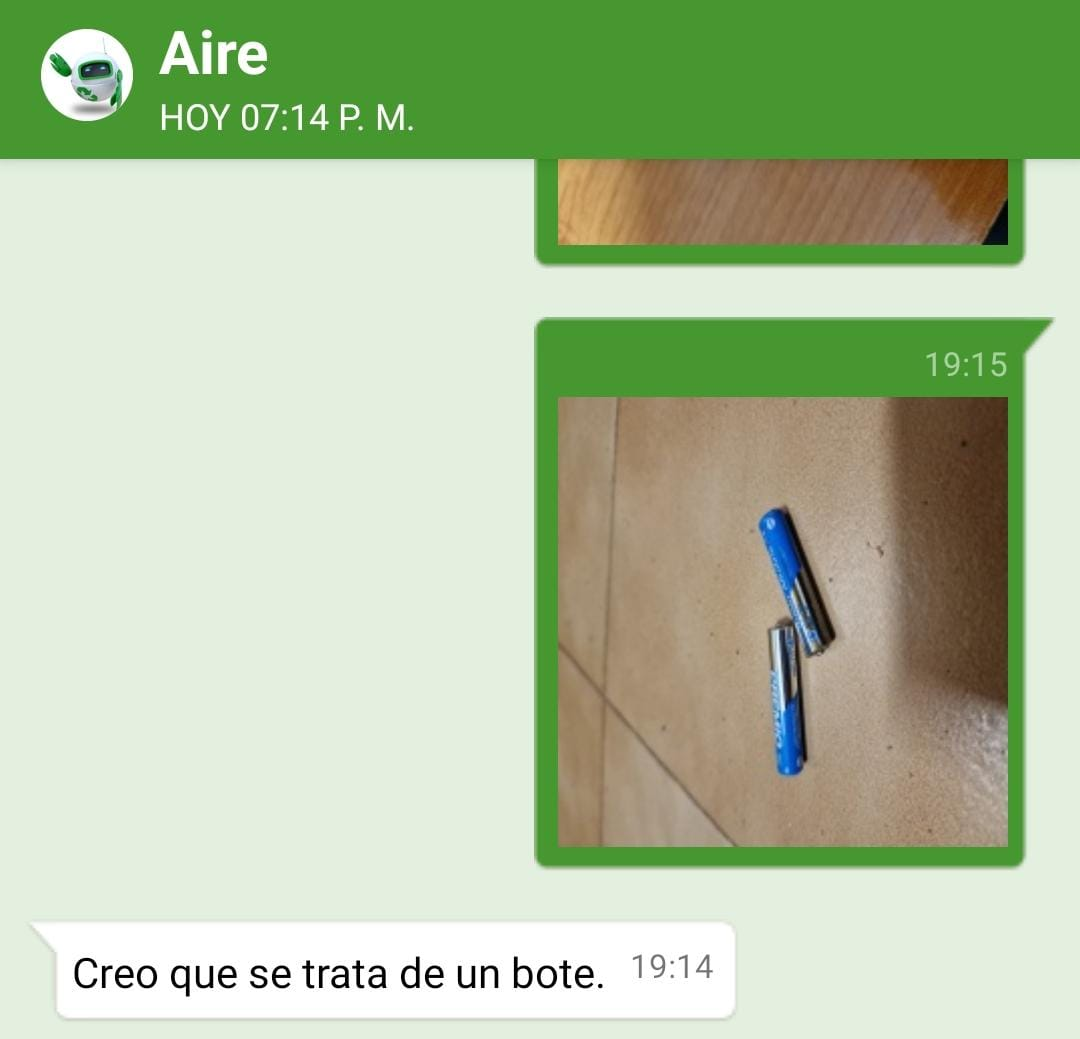
\includegraphics[scale=0.2]{img/aire.jpeg}
  \caption{Aplicación Aire en funcionamiento}
  \label{fig:aire}
\end{figure}

En este trabajo de investigación, se abordarán diversas cuestiones relacionadas con la clasificación de residuos utilizando técnicas de inteligencia artificial.

Para aportar soluciones a este problema, se han definido los siguientes objetivos:

\begin{enumerate}
\item Generar un gran dataset para cubrir la mayor cantidad de residuos reciclables y no reciclables utilizando utilizando una aplicación móvil para etiquetar de manera más colaborativa.
\item Facilitar el reciclaje de residuos utilizando una aplicación móvil que permita a los usuarios clasificar sus residuos de manera automática superando las aplicaciones domésticas actuales.
\item Explorar la viabilidad de generar un dataset semántico a partir de uno de clasificación, para reducir el tiempo y coste del etiquetado.
\end{enumerate}

Con estos objetivos se busca mejorar la clasificación de residuos y contribuir a la gestión sostenible de los mismos.

\section{Estado del Arte}

En este apartado se ha realizado una revisión de los trabajos más relevantes en el campo de la clasificación de imágenes.

\subsection{Clasificación}

En los últimos años, se han logrado importantes avances en el campo del Deep Learning, esto gracias a la aparición
de los Transformers. Presentados en el paper de Attention is all you need \cite{transformers}.

Los Transformers son clave en modelos de inteligencia artificial porque han demostrado ser muy efectivos en tareas
de procesamiento del lenguaje natural (NLP, por sus siglas en inglés) y otras aplicaciones relacionadas con el
aprendizaje automático, incluso extrapolando su uso a todo tipo de tareas. Pero antes de que los Transformers
se convirtieran en la base de los modelos de inteligencia artificial, las redes neuronales convolucionales (CNN) y
las redes neuronales recurrentes (RNN) eran las arquitecturas más utilizadas para resolver problemas de clasificación
de imágenes y procesamiento del lenguaje natural, respectivamente.

\subsubsection{Visión por Computador Clásica}

La visión por computador clásica es un área que se centra en la interpretación y manipulación de imágenes digitales. El principal objetivo de esta disciplina es emular la visión humana utilizando técnicas de procesamiento de imágenes y aprendizaje automático. El proceso clásico de reconocimiento de imágenes se basa principalmente en dos pasos: la extracción de características y el aprendizaje automático.

\begin{itemize}
    \item \textbf{Extracción de Características:} Esta etapa implica la transformación de las imágenes en un conjunto de características que describen la imagen en cuestión. Las técnicas utilizadas pueden ser tan simples como el color, la textura y la forma, hasta métodos más complejos como el Histograma de Gradientes Orientados (HOG) \cite{hog}, SIFT \cite{SIFT}, SURF \cite{SURF}, entre otros. Este proceso es crucial para preparar los datos para el siguiente paso, el aprendizaje automático.
    \item \textbf{Machine Learning:} En la fase de aprendizaje automático, se utilizan los descriptores de la imagen, extraídos en la etapa anterior, para entrenar un modelo que pueda reconocer o clasificar imágenes. Algunos ejemplos comunes de estos modelos son Support Vector Machines (SVM) \cite{svm}, k-Nearest Neighbors (k-NN), y Random Forest \cite{random_forest}.
\end{itemize}

\subsubsection{Redes Neuronales}

Las redes neuronales artificiales son un modelo de aprendizaje profundo que intenta simular la forma en que el cerebro humano funciona. Aunque los modelos de red neuronal se introdujeron por primera vez en la década de 1940, no fue hasta la década de 1980 que se popularizaron con la introducción del algoritmo de retropropagación. A continuación, se proporciona un resumen de los modelos de redes neuronales más utilizados en la clasificación de imágenes:

\begin{itemize}
    \item \textbf{MLP (Multilayer Perceptron):} El MLP es una red neuronal que consta de al menos tres capas de nodos: una capa de entrada, una o más capas ocultas, y una capa de salida. Cada nodo está conectado a todos los demás nodos de la siguiente capa, formando una red interconectadas de nodos.
    \item \textbf{CNN (Convolutional Neural Network):} Las CNN son una categoría especializada de redes neuronales que han demostrado ser muy eficaces en tareas de reconocimiento y clasificación de imágenes. Las CNN utilizan una variedad de capas, como capas convolucionales, de pooling y fully-connected, para procesar imágenes. La idea detrás de las CNN es que no es necesario diseñar manualmente los extractores de características, en su lugar, la red aprende estas características por sí misma durante el entrenamiento. 
  \end{itemize}

\subsubsection{Convolutional Neural Networks en detalle}

Las Convolutional Neural Networks (CNN) han revolucionado el campo de la visión por computador desde su introducción. Estos modelos se basan en el concepto de convolución, que es una operación matemática que permite procesar una imagen con un filtro o kernel. Este proceso permite a la CNN detectar características locales en las primeras capas, como bordes y texturas, mientras que en las capas más profundas, la red puede detectar características más abstractas, como partes de objetos o incluso objetos completos.

Una de las mayores ventajas de las CNN es su capacidad para manejar imágenes de alta resolución. A diferencia de las redes neuronales tradicionales, donde el número de parámetros aumenta drásticamente con el tamaño de la imagen, las CNN mantienen un número manejable de parámetros al compartir pesos a través de la convolución.

Los modelos de CNN han evolucionado con el tiempo, y han surgido numerosas arquitecturas con rendimientos sobresalientes. Algunos ejemplos notables incluyen:

\begin{itemize}
    \item \textbf{LeNet \cite{lenet}:} Propuesto por LeCun et al. en 1998, fue una de las primeras CNN exitosas y fue diseñada para reconocer dígitos escritos a mano.
    \item \textbf{AlexNet \cite{alexnet}:} Propuesto por Krizhevsky et al. en 2012, ganó la competencia ImageNet y estableció a las CNN como la principal técnica para la clasificación de imágenes.
    \item \textbf{VGGNet \cite{vgg}:} Propuesto por Simonyan y Zisserman en 2014, introdujo la idea de redes más profundas con muchas capas convolucionales. 
    \item \textbf{ResNet \cite{resnet}:} Propuesto por He et al. en 2015, introdujo las conexiones residuales que permiten entrenar redes extremadamente profundas.
\end{itemize}

Las CNN continúan siendo una área activa de investigación, y se están desarrollando nuevas arquitecturas y técnicas para mejorar aún más su rendimiento en la clasificación de imágenes.

\subsubsection{CLIP}

La clasificación ha dado un cambio radical con la salida del CLIP (Contrastive Language–Image Pre-training) \cite{clip}. CLIP es un modelo de aprendizaje profundo que ha cambiado el estado del arte en la clasificación de imágenes. Utiliza un modelo de lenguaje para entender tanto las imágenes como el texto relacionado y una técnica de aprendizaje por similitud para clasificar imágenes en función de su similitud con una determinada descripción textual.

\begin{figure}[h]
  \centering
  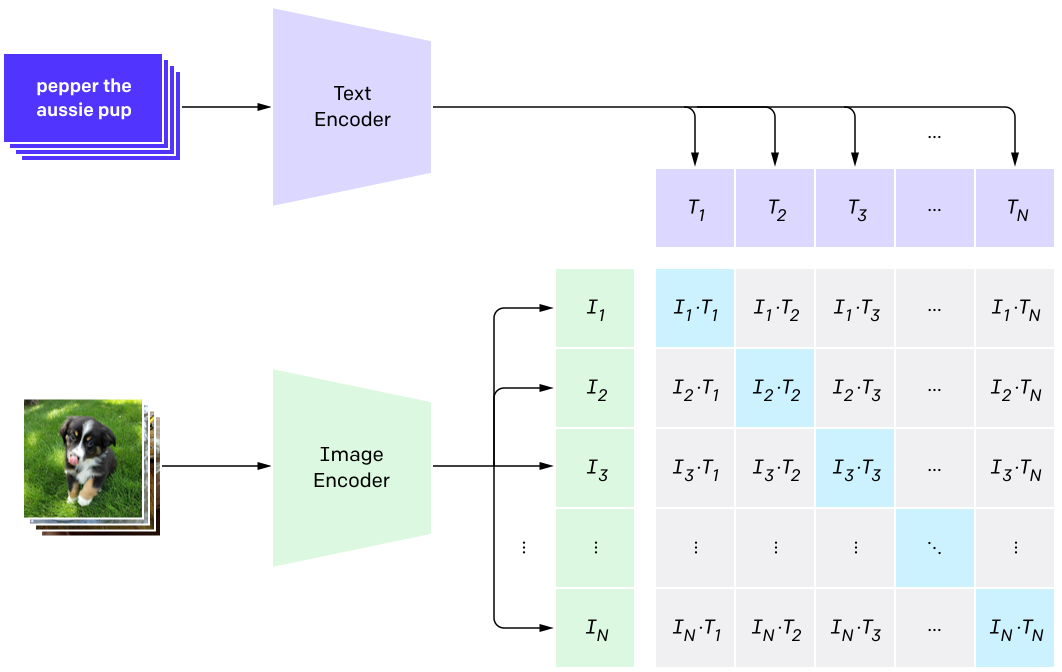
\includegraphics[scale=0.2]{img/CLIP_diagram.png}
  \caption{Arquitectura de CLIP, creada por OpenAI.}
\end{figure}

En comparación con los modelos clásicos de redes neuronales convolucionales, CLIP puede comprender el contexto y el significado detrás de una imagen, lo que lo hace especialmente útil en situaciones en las que las imágenes pueden ser difíciles de clasificar para los modelos clásicos.

\begin{table}[h]
  \centering
  \begin{tabular}{llll}
    \toprule
    \textbf{Modelos}     & \textbf{Accuracy} & \textbf{Params} & \textbf{Tecnology} \\ 
    \midrule
    BASIC-L            & 91.1\%            & 2440M           & Conv+Transf	    \\
    CoCa               & 91.0\%            & 2100M           & Transformer        \\
    Model soups        & 90.98\%           & 2440M           & Conv+Transf	    \\
    Model soups        & 90.94\%           & 1843M           & Transformer        \\
    ViT-e              & 90.9\%            & 3900M           & Transformer        \\
    CoAtNet-7          & 90.88\%           & 2440M           & Conv+Transf	    \\
    ViT-G/14           & 90.71\%           & 1843M           & Transformer        \\
    CoCa               & 90.60\%           & 2100M           & Transformer        \\
    CoAtNet-6          & 90.45\%           & 1470M           & Conv+Transf	    \\
    ViT-G/14           & 90.45\%           & 1843M           & Transformer        \\
    DaViT-G            & 90.4\%            & 1437M           & Transformer        \\
    Meta Pseudo Labels & 90.2\%            & 480M            & EfficientNet       \\
    DaViT-H            & 90.2\%            & 362M            & Transformer        \\
    SwinV2-G           & 90.17\%           & 3000M           & Transformer        \\
    Florence-CoSwin-H  & 90.05\%           & 893M            & Transformer        \\
    Meta Pseudo Labels & 90\%              & 390M            & EfficientNet       \\
    RevCol-H           & 90.0\%            & 2158M           & Pure CNN           \\
    \bottomrule
  \end{tabular}
  \caption{Comparativa de modelos de clasificación con mejor accuracy en imágenes del dataset Imagenet Tabla extraída y adaptada de "paperswithcode". Modelos del 2020 al 2023-Q1.}
  \label{tab:clasificacion}
\end{table}

En la Tabla \ref{tab:clasificacion} se puede ver una comparativa de los modelos de clasificación de
imágenes más destacados del 2020 al 2023-Q1 y como los modelos basados en Transformers (entrenados con el contexto) son superiores
a los son puramente convolucionales. Esto se debe a que los modelos de redes
neuronales convolucionales puros no pueden comprender el contexto y el significado detrás de
una imagen, mientras que los modelos de redes neuronales basados en Transformer pueden
comprender el contexto y el significado detrás de una imagen consiguiendo mejores resultados.

\subsection{Visualización de Redes Neuronales}

La visualización de las redes neuronales se ha vuelto esencial para comprender los modelos de aprendizaje profundo. Existen diversas técnicas destacadas en este campo.

\subsubsection{Mapas de Activación de Clase}

El mapa de activación de clase (CAM) es una técnica de visualización de características que permite visualizar qué partes de una imagen son importantes para una clase en particular. CAM se puede utilizar para cualquier red neuronal convolucional (CNN) con una capa de agrupación global (GAP) en la parte superior.\\

\begin{itemize}
    \item \textbf{GradCAM \cite{grad_cam}}: Utiliza los gradientes de cualquier capa objetivo para producir un mapa de activación de clase. GradCAM utiliza los gradientes de la clase de salida con respecto a las características de la capa para ponderar la importancia de cada característica para la decisión de la clase.
    \item \textbf{ScoreCAM \cite{ScoreCAM}}: Se basa en una serie de modificaciones del enfoque original de GradCAM para evitar problemas de localización. En lugar de utilizar gradientes, ScoreCAM ajusta cada canal de características de la capa objetivo y pasa las imágenes ajustadas a través de la red para obtener puntuaciones.
    \item \textbf{LayerCAM \cite{LayerCAM}}: Combina la evidencia de múltiples capas de la red para generar un mapa de activación de clase más preciso. LayerCAM introduce un factor de ponderación que da más importancia a las características de alto nivel en comparación con las características de bajo nivel.
\end{itemize}

\subsubsection{Mapas de Saliencia}

Los mapas de Saliencia son una técnica de visualización de características que permite visualizar qué partes de una imagen son importantes para una clase en particular. Los mapas de Saliencia se pueden utilizar para cualquier (CNN).\\

\begin{itemize}
    \item \textbf{Saliency Map \cite{SalencyMap}}: Para calcular un mapa de Saliencia, lo que se hace es calcular la derivada (o gradiente) de la salida de la red con respecto a la entrada. Este cálculo indica cuánto cambiaría la salida de la red si se cambia ligeramente un píxel en la imagen de entrada. Si este cambio es grande,
    entonces ese píxel es importante para la clasificación de la red, y se decolorará fuertemente en el mapa de Saliencia. Si este cambio es pequeño, entonces ese píxel no es muy importante para la clasificación de la red, y será menos colorido en el mapa de Saliencia. Este tipo de técnica suele generar ruido en la salida, es decir puede haber pixeles que no sean importantes pero que se coloreen fuertemente generando inconsistencias.
    \item \textbf{SmoothGrad \cite{SmoothGrad}}: Es una técnica que se utiliza para mejorar la calidad y la interpretación de los mapas de Saliencia generados por las redes neuronales. Los mapas de Saliencia pueden ser ruidosos o inconsistentes.
    Para superar este problema, SmoothGrad introduce ruido gaussiano a las entradas de la red. El ruido gaussiano es esencialmente una perturbación aleatoria con cierta variabilidad, que se añade a cada pixel de la imagen de entrada.
    Este proceso de añadir ruido se repite muchas veces, y para cada versión con ruido de la imagen, se calcula un mapa de Saliencia. Luego, estos mapas se promedian para obtener un mapa de Saliencia "suavizado".
    El resultado de este proceso es un mapa de Saliencia más suave y menos ruidoso, que puede ser más fácil de interpretar y entender.
\end{itemize}

A medida que los modelos de aprendizaje profundo se vuelven cada vez más complejos, las técnicas de visualización y los algoritmos se vuelven cada vez más necesarios para interpretar estos modelos.

Por lo general los mapas de Saliencia suele ser más precisos que los mapas de activación de clase, pero son más costosos computacionalmente.

\subsection{Segmentación Semántica}

La segmentación semántica es una tarea de clasificación de píxeles que tiene como objetivo asignar a cada píxel en una imagen una etiqueta de clase específica. Formalmente, dada una imagen de entrada $I$ de tamaño $W \times H \times C$ (donde $W$ es el ancho, $H$ es la altura y $C$ son los canales de color), el objetivo es generar un mapa de segmentación $S$ de tamaño $W \times H$ donde cada ubicación $s_{ij}$ en $S$ contiene la etiqueta de clase de la ubicación correspondiente en la imagen de entrada.

Los métodos convencionales para la segmentación semántica incluyen técnicas como el crecimiento de regiones y la segmentación por aguas divisorias. Sin embargo, con el surgimiento de las redes neuronales convolucionales (CNNs), los enfoques basados en el aprendizaje profundo se han convertido en el estándar de oro para la segmentación semántica.

Uno de los modelos más influyentes en este campo es la Red SegNet, que es una arquitectura de red neuronal convolucional completamente convolucional para la segmentación semántica. La arquitectura de SegNet se puede describir como sigue: dada una imagen de entrada $I$, se aplica una serie de capas convolucionales para producir una representación de características $F$ de tamaño reducido. Luego, se aplica un conjunto de capas de decodificación a $F$ para producir el mapa de segmentación de salida $S$.

La función de pérdida que se utiliza comúnmente para entrenar estos modelos es la entropía cruzada, que se puede observar en la Ecuación \ref{eq:crossentropy}.

\begin{equation}
L(\theta) = -\frac{1}{N}\sum_{i=1}^{N}\sum_{j=1}^{J} y_{ij} \log(\hat{y}_{ij})
\label{eq:crossentropy}
\end{equation}

donde $N$ es el número de píxeles en la imagen, $J$ es el número de clases, $y_{ij}$ es la etiqueta de clase real para el píxel $i$ en la clase $j$, y $\hat{y}_{ij}$ es la probabilidad predicha por el modelo para el píxel $i$ en la clase $j$.

Los modelos modernos de segmentación semántica, como U-Net \cite{unet}, Mask R-CNN \cite{maskrcnn} y DeepLab \cite{deeplab}, han extendido y mejorado estas ideas básicas, proporcionando un rendimiento de segmentación semántica de vanguardia en una variedad de tareas y dominios.

\section{Desarrollo}

En esta sección se explica el desarrollo del proyecto, desde la creación del dataset hasta la publicación de la aplicación móvil en la Play Store.

\subsection{Dataset}

Unos de los principales problemas para la generación del dataset es que en cada región tiene un sistema de
reciclaje diferente y por lo tanto las clases de residuos que se pueden reciclar también son diferentes por lo que
ha sido necesario crear un dataset propio adaptado a Cataluña. El motivo de utilizar el sistema de Cataluña
es porque llevan tiempo fomentando la separación de residuos y hay mucha información disponible sobre el tema.

Residuonvas.cat es una página web que tiene como objetivo informar a la población sobre la gestión de residuos
en Cataluña. En su sitio web, promueven un sistema de clasificación y separación de residuos en diferentes
categorías para su posterior tratamiento y reciclaje. A continuación, se presenta una lista de las diferentes
clases de residuos para reciclar que se promueven en este sistema:

\setlength{\columnsep}{0cm}
\begin{center}
\begin{multicols}{2}
  \begin{itemize}[noitemsep, leftmargin=*]
  \item[] Envase de vidrio
  \item[] Medicamentos
  \item[] Aparatos eléctricos
  \item[] Punto verde
  \columnbreak
  \item[] Envase ligero
  \item[] Pilas y baterías
  \item[] Ropa y calzado
  \item[] Orgánica
  \item[] Resta
  \end{itemize}
  \end{multicols}
\end{center}

Esta lista serán las clases que se utilizaran para la creación del dataset. A lo largo del paper se ha utilizado
el contenedor donde se deposita el residuo para referirse a la clase, por ejemplo, en vez de decir que se ha
clasificado un residuo como envase de vidrio se dirá que se ha clasificado como verde.

Para la recolección del dataset se ha utilizado diferentes dataset de residuos para tener una base solida para poder
entrenar el modelo. También se ha desarrollado una aplicación móvil para la recolección de imágenes de residuos
y así obtener un dataset más completo y concreto de residuos domésticos. En la Tabla \ref{tab:dist_clases} se puede ver
la distribución de las clases en el dataset.

\begin{table}[h]
  \centering
  \begin{tabular}{l|ll|ll|l}
  \toprule
  Clase & Train & \%  & Val & \%  & Total \\ 
  \midrule
  Amarillo       & 7371           & 15.15        & 500          & 10.64        & 7871           \\
  Azul           & 4230           & 8.7          & 500          & 10.64        & 4730           \\
  Marron         & 4980           & 10.24        & 500          & 10.64        & 5480           \\
  Medicamento    & 3156           & 6.49         & 400          & 8.51         & 3556           \\
  Pilas          & 3214           & 6.61         & 300          & 6.38         & 3514           \\
  Punto          & 4576           & 9.41         & 500          & 10.64        & 5076           \\
  RAEE           & 6258           & 12.87        & 500          & 10.64        & 6758           \\
  Resta          & 4443           & 9.13         & 500          & 10.64        & 4943           \\
  Ropa           & 5332           & 10.96        & 500          & 10.64        & 5832           \\
  Verde          & 5081           & 10.45        & 500          & 10.64        & 5581           \\
  \midrule
  Total & 48641 & 100 & 4700 & 100 & 53341 \\
  \bottomrule
  \end{tabular}
  \caption{Distribución de las clases y en los conjuntos de entrenamiento y validación}
  \label{tab:dist_clases}
\end{table}

El motivo de no tener los datos de test es porque se ha esperado a que los usuarios de la aplicación móvil
contribuyan con más imágenes para poder tener un dataset más completo y concreto de residuos domésticos.

Para la búsqueda del mejor modelo de momento se utilizará el conjunto de validación. Una vez seleccionado el
mejor modelo se utilizará el conjunto de test para ver el rendimiento del modelo en un conjunto de datos que
provienen de usos domésticos reales, aportando una auténtica perspectiva práctica a nuestro análisis.

\begin{figure}[h]
  \centering
  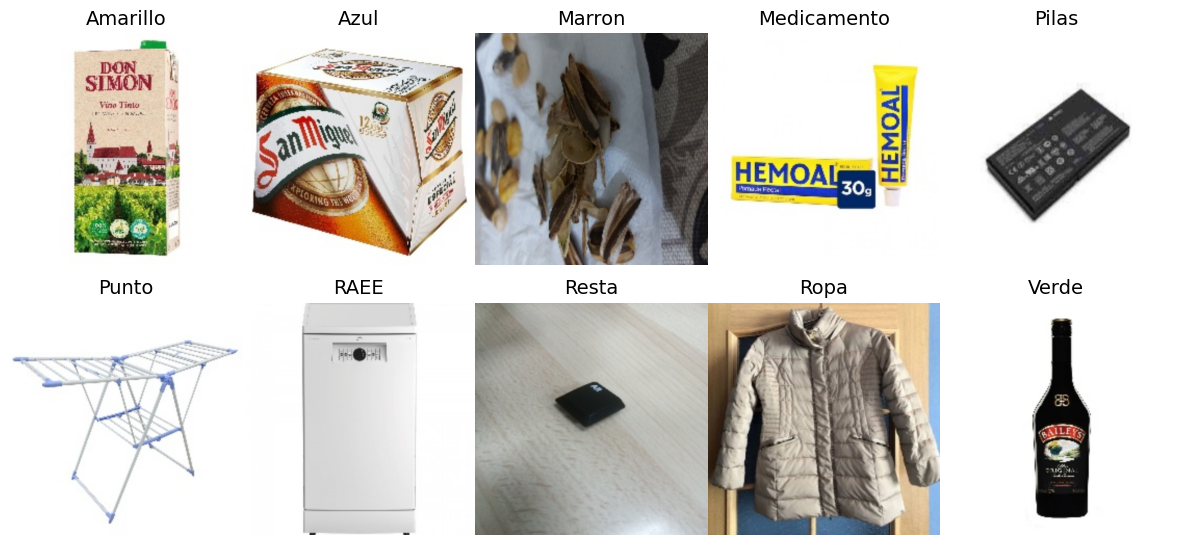
\includegraphics[width=0.50\textwidth]{img/imagenes.png}
  \caption{Imágenes de cada clase extraídas del conjunto de entrenamiento.}
  \label{fig:imagenes_clases}
\end{figure}

En la Figura \ref{fig:imagenes_clases} se puede ver una imagen de cada clase extraída del conjunto de entrenamiento.

\subsection{Aplicación móvil}

Para poder recolectar imágenes domésticas reales de residuos se ha desarrollado una aplicación móvil para Android llamada EcoMate.

Ha sido diseñada para permitir a los usuarios contribuir y mantener un dataset de imágenes en tiempo real de manera sencilla.
EcoMate fomenta la colaboración y el aprendizaje en torno a la clasificación y manejo de residuos.

Las principales funcionalidades de la aplicación son:

\begin{enumerate}
  \item Listado en tiempo real: EcoMate muestra la cantidad de imágenes que los usuarios han contribuido al dataset, permitiendo a los usuarios mantenerse actualizados sobre el progreso de la comunidad.
  \item Ranking de contribuyentes: La aplicación incluye un ranking que muestra la cantidad total de imágenes que ha contribuido el usuario en el primer puesto, fomentando la competencia amistosa y el compromiso con la plataforma.
  \item Visualización de la última imagen: Los usuarios pueden ver la última imagen con la que han contribuido, lo que les permite revisar su progreso y mantenerse al tanto de sus aportaciones al dataset.
  \item Carga de imágenes desde la cámara: EcoMate permite a los usuarios agregar imágenes nuevas directamente desde la cámara de su dispositivo móvil. Una vez tomada la foto, se asigna una clase del dataset y se carga en el servidor, actualizando automáticamente los datos en tiempo real.
  \item Autenticación y seguridad: La aplicación utiliza Firebase como backend, con módulos de autenticación, Firestore Database, Storage y Realtime Database activos. Además, EcoMate ofrece inicio de sesión y registro con correo electrónico, verificación de correo electrónico y funcionalidad de ``olvidé mi contraseña'' para garantizar la seguridad y privacidad de los usuarios.
  \item Clasificación de imágenes: La aplicación permite clasificar la imagen que se ha tomado con la cámara del dispositivo móvil e indicar en que contenedor se debe depositar.
  \item Imágenes similares: La aplicación permite ver imágenes similares a la que se ha tomado con la cámara del dispositivo móvil.
\end{enumerate}

Desde que estuvo disponible en la Play Store, se ha recolectado un total de 398 imágenes de residuos.

\begin{figure}[h]
  \centering
  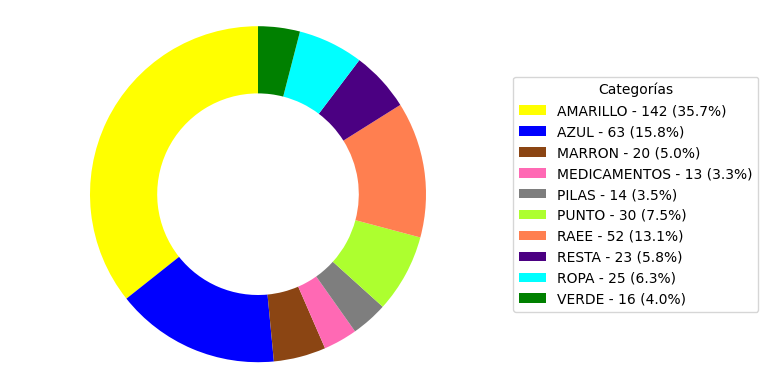
\includegraphics[width=0.45\textwidth]{img/distribucion_app.png}
  \caption{Distribución de las clases en el dataset de la aplicación.}
  \label{fig:distribucion_app}
\end{figure}

Como se puede observar en la Figura \ref{fig:distribucion_app} la clase con más imágenes es la de AMARILLO, con 142 imágenes, mientras que la clase con menos imágenes es la de MEDICAMENTO. Esta información puede proporcionar una idea de cuáles son las clases más fáciles de obtener imágenes y cuáles son las más difíciles.

\subsection{Modelo de clasificación}

El principal objetivo de esta sección es identificar y seleccionar el modelo óptimo para llevar a cabo la clasificación de residuos de manera eficaz y precisa. Para lograrlo, se ha empleado la plataforma TensorFlow V2, en conjunto con la API de Keras, la cual facilita el diseño, entrenamiento y evaluación de modelos de aprendizaje profundo. Asimismo, se ha utilizado una tarjeta gráfica NVIDIA RTX 3060 con 12 GB de memoria de vídeo, permitiendo agilizar el proceso de entrenamiento y mejorar el rendimiento de los modelos.

En todas las pruebas realizadas se han usado los paramentos de la Tabla \ref{table:hyperparameters}.

\begin{table}[h]
  \centering
  \begin{tabular}{|l|l|}
  \hline
  \textbf{Hiperparámetro} & \textbf{Valor} \\ \hline
  Optimizador & Adam \\ \hline
  Learning rate & 0.001 \\ \hline
  Amsgrad & True \\ \hline
  Loss & Categorical crossentropy \\ \hline
  Early stopping & Monitor: val\_loss, Patience: 4 \\ \hline
  ModelCheckpoint & Monitor: val\_loss, Save best only: True \\ \hline
  Número de épocas & Hasta converger \\ \hline
  \end{tabular}
  \caption{Hiperparámetros utilizados en las pruebas.}
  \label{table:hyperparameters}
\end{table}

Se realizaron las primeras pruebas, Tabla \ref{table:simple_models}, utilizando modelos simples, como una red neuronal multicapa (MLP) y una red neuronal convolucional (CNN). Estos modelos se entrenaron utilizando el conjunto de datos de entrenamiento sin realizar ninguna modificación en las imágenes.

Los valores analizados para evaluar el rendimiento de los modelos fueron la precisión con los datos de validación (Acc), la pérdida con los datos de validación (Loss), el número de parámetros (Params), el número de épocas (Epo) y el tiempo de ejecución por época en segundos (T/Epo).

\begin{table}[h]
  \centering
  \begin{tabular}{@{}llllll@{}}
    \toprule
    \textbf{Modelo} & \textbf{Acc} & \textbf{Loss} & \textbf{Params} & \textbf{Epo} & \textbf{Time/Epoch} \\
    \midrule
    simple\_cnn & 0.54 & 3.78 & 44.4M & 7 & 184.61 \\
    simple\_mlp & 0.33 & 1.95 & 77.24M & 22 & 71.35 \\
    \bottomrule
  \end{tabular}
  \caption{Resultados de las pruebas con modelos simples.}
  \label{table:simple_models}
\end{table}

El modelo de red neuronal convolucional (CNN) ha demostrado un rendimiento superior como se observa en la Tabla \ref{table:simple_models}, ya que, al trabajar con imágenes, las CNN superan a las redes neuronales multicapa (MLP). Además, se observa que el modelo CNN requiere un tiempo de entrenamiento por época significativamente mayor que el modelo MLP, a pesar de tener menos parámetros. Esto se debe a que el entrenamiento de capas convolucionales es mucho más costoso que el de capas densas. Sin embargo, el modelo CNN ha necesitado menos épocas para converger. Los resultados de esta primera prueba nos indican que no es posible desarrollar un modelo de clasificación con una precisión aceptable si optamos por utilizar una red neuronal convolucional.

En la segunda prueba, se han utilizado modelos preentrenados con el conjunto de datos ImageNet. Para esta prueba inicial, se han congelado las capas de la red preentrenada y se han añadido una capa densa de 1024 neuronas y una capa de salida con 10 neuronas. De esta manera, podemos aprovechar el conocimiento previo de la red preentrenada y entrenar únicamente las capas añadidas.

\begin{table}[h]
  \centering
  \label{table:pretrained_models}
  \begin{tabular}{@{}lccccc@{}}
    \toprule
    \textbf{Model}                      & \textbf{Acc} & \textbf{Loss} & \textbf{Params} & \textbf{Epo} & \textbf{T/Epo} \\
    \midrule
    xception\cite{chollet2017xception}                            & 0.83              & 0.69          & 123.63M         & 5               & 280.99              \\
    inceptionresnetv2\cite{szegedy2017inception}                   & 0.83              & 0.78          & 93.67M          & 6               & 510.01              \\
    nasnetmobile\cite{Zoph2018}                        & 0.81              & 0.73          & 57.27M          & 4               & 263.30              \\
    resnet50v2\cite{he2016identity}                          & 0.81              & 1.10          & 126.34M         & 4               & 291.10              \\
    mobilenetv2\cite{sandler2018mobilenetv2}                         & 0.80              & 1.06          & 66.49M          & 4               & 114.87              \\
    vgg16\cite{vgg16}                               & 0.74              & 1.36          & 40.42M          & 8               & 221.76              \\
    convnexttiny\cite{Liu2020conv}                        & 0.53              & 1.67          & 66.37M          & 6               & 727.44              \\
    \bottomrule
  \end{tabular}
  \caption{Resultados de las pruebas con modelos pre-entrenados y las capas convolucionales congeladas.}
  \label{table:pretrained_models}
\end{table}

Si observamos la Tabla \ref{table:pretrained_models} la mayoría de los modelos preentrenados han logrado una precisión superior al 80\%, lo que demuestra que el conocimiento adquirido a partir de las imágenes de ImageNet es de gran utilidad para clasificar las imágenes de nuestro conjunto de datos.

Cabe destacar que los modelos preentrenados requirieron menos épocas para converger en comparación con modelos anteriores. Esto se debe a que las capas convolucionales de los modelos preentrenados ya han aprendido a extraer características de las imágenes, por lo que solo necesitan aprender a clasificar las características extraídas.

Es importante mencionar que, a pesar de ser un modelo preentrenado, el modelo convnexttiny obtuvo una precisión muy baja en comparación con los demás.

En la tercera prueba, se llevó a cabo un entrenamiento completo de los modelos preentrenados, lo que implica descongelar las capas convolucionales y entrenar todo el modelo.

Para llevar a cabo este entrenamiento, se congelaron todas las capas convolucionales y se entrenaron únicamente la capa densa y la capa de salida durante cinco épocas. Posteriormente, se descongelaron todas las capas convolucionales y se entrenó todo el modelo hasta alcanzar la convergencia.

Además, se implementó el aumento de datos (``Data Augmentation'') debido a que, al descongelar todas las capas convolucionales, se incrementó el número de parámetros entrenables. Esto hace necesario aumentar el número de datos de entrenamiento para evitar el sobreajuste (``overfitting'').

Las transformaciones aplicadas incluyen: rotación, traslación, volteo horizontal y ajuste aleatorio de brillo y contraste.

Se optó por utilizar un aumento de datos en tiempo real y diferente para cada iteración, aplicando transformaciones aleatorias a las imágenes de entrenamiento. Las probabilidades (p) de aplicar cada transformación son:

\begin{itemize}[noitemsep]
  \item[] Rotación: p = 0.5
  \item[] Traslación: p = 0.5
  \item[] Flip horizontal: p = 0.5
  \item[] Random brightness and contrast: p = 0.5
\end{itemize}

Es decir que, en cada iteración, la imagen de entrada pasa por un pipeline de transformaciones aleatorias con las probabilidades indicadas anteriormente,
primero se aplica una rotación aleatoria de 0 a 45 grados en caso de que la probabilidad sea mayor a 0.5, luego se aplica una traslación aleatoria de 0 a 0.2 en caso de que la probabilidad sea mayor a 0.5,
así sucesivamente hasta que se aplican todas las transformaciones.

En la Tabla \ref{table:pretrained_models_unfrozen} se muestran los resultados sin tener en cuenta el tiempo de entrenamiento de las 5 primeras épocas.

\begin{table}[h]
  \centering
  \begin{tabular}{@{}llllll@{}}
    \toprule
    \textbf{Modelo}        & \textbf{Acc} & \textbf{Loss} & \textbf{Params} & \textbf{Epo} & \textbf{T/Epo} \\ 
    \midrule
    convnexttiny           & 0.91         & 0.36          & 66.37M          & 12           & 1799.02        \\
    xception               & 0.90         & 0.36          & 123.63M         & 10           & 670.20         \\
    inceptionresnetv2      & 0.90         & 0.38          & 93.67M          & 10           & 1149.01        \\
    nasnetmobile           & 0.87         & 0.54          & 57.27M          & 13           & 789.63         \\
    resnet50v2             & 0.86         & 0.54          & 126.34M         & 17           & 649.03         \\
    mobilenetv2            & 0.88         & 0.44          & 66.49M          & 15           & 358.09         \\
    vgg16                  & 0.84         & 0.56          & 40.42M          & 22           & 689.81         \\
    \bottomrule
  \end{tabular}
  \caption{Resultados de las pruebas con modelos pre-entrenados y las capas convolucionales descongeladas.}
  \label{table:pretrained_models_unfrozen}
\end{table}

Tres modelos de los siete mostrados han obtenido un accuracy superior al 90\% y lo más importante es que el
accuracy de convnexttiny ha mejorado considerablemente.

Finalmente se ha realizado una prueba con los modelos pre-entrenados sin ``Data Augmentation'' para comparar los resultados
y demostrar que el ``Data Augmentation'' es necesario para obtener buenos resultados.

\begin{table}[h]
  \centering
  \begin{tabular}{llllll}
    \toprule
    \textbf{Modelo}               & \textbf{Acc} & \textbf{Loss} & \textbf{Epo} & \textbf{T/Epo} \\ 
    \midrule
    Xception aug              & 0.90              & \textbf{0.36}                    & 10             & 670.20              \\
    Xception no aug              & 0.90              & 0.53                   & 6              & 808.19              \\
    \midrule
    MobileNetV2 aug           & 0.88              & \textbf{0.44}                      & 15             & 358.09              \\
    MobileNetV2 no aug           & 0.88              & 0.70                      & 10             & 335.72              \\
    \bottomrule
  \end{tabular}
  \caption{Comparativa de modelos usando y sin usar ``Data Augmentation''.}
  \label{table:pretrained_models_aug}
\end{table}

Realizar ``Data Augmentation'' hace que el loss sea menor, ver Tabla \ref{table:pretrained_models_aug}, esto quiere decir que el modelo es más robusto
y sera menos propenso al sobre-ajuste y generalizará mejor.

Sobre el tiempo de inferencia de los modelos, se ha realizado una prueba con una imagen y se ha medido el tiempo que tarda
cada modelo en realizar la predicción.

\begin{figure}[h]
  \centering
  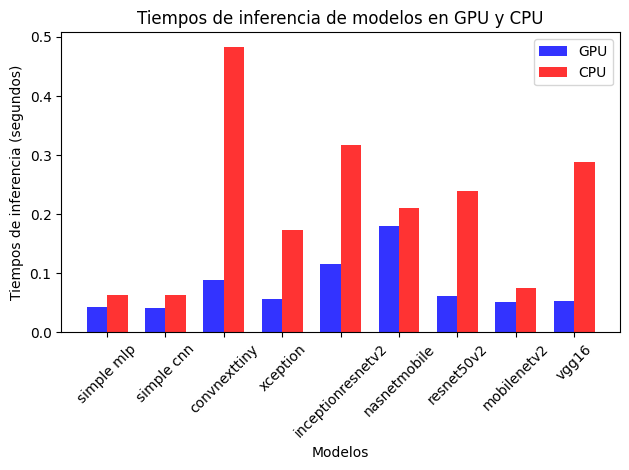
\includegraphics[width=0.4\textwidth]{img/comparativa modelos.png}
  \caption{Tiempos de inferencia de los modelos.}
  \label{fig:infertime}
\end{figure}

Es interesante analizar el tiempo de inferencia al desplegar un modelo en un dispositivo de bajo rendimiento, como un dispositivo móvil o un dispositivo IoT. Como se
mustra en la Figura \ref{fig:infertime}, el modelo mas beneficiado es el modelo convnexttiny.

\subsection{CLIP}

CLIP es una tecnología con habilidades zero-shot muy potentes y que nos puede ser útil para proporcionar información adicional al usuario sobre la imagen que ha subido y también para clasificar
imágenes. Para ello se ha realizado un listado de las clases que quieres clasificar que se encuentran en la pagina \href{https://www.residuonvas.cat/ca}{ResiduOnVas} siendo un total de 247 clases.

La implementación de CLIP que se ha utilizado ha sido OpenCLIP con la variante ViT-g/14.

Estos modelos son altamente sensibles a la formulación del prompt de salida, por lo que se han realizado pruebas con distintas formulaciones para ver cual es la que mejor se adapta al dataset, este tipo
de pruebas se empiezan a conocer como \textit{Prompt Engineering}.

\begin{table}[h]
  \centering
  \begin{tabular}{@{}lrr@{}}
  \toprule
  \textbf{Prompt}                                                 & \textbf{acc}              & \textbf{std}              \\ \midrule
  \{\}                                                   & 0.707          & 0.158          \\
  \midrule
  a photo of \{\}                                        & 0.753          & 0.140          \\
  a picture of \{\}                                      & 0.730          & 0.171          \\
  a photo of a \{\}                                      & 0.760           & 0.144          \\
  a picture of a \{\}                                    & 0.747          & 0.151          \\
  an image of \{\}                                       & 0.759          & 0.152          \\
  an image of a \{\}                                     & 0.762           & 0.152          \\
  a bright photo of a \{\}                               & 0.745          & 0.147          \\ 
  \midrule
  a photo of \{\}, a type of waste                       & 0.761          & 0.111          \\
  a picture of \{\}, a type of waste                     & 0.760          & 0.115          \\
  a photo of a \{\}, a type of waste                     & 0.778          & 0.105          \\
  a picture of a \{\}, a type of waste                   & 0.782          & 0.106          \\
  an image of \{\}, a type of waste                      & 0.757          & 0.113          \\
  an image of a \{\}, a type of waste                    & 0.779          & 0.109          \\
  a bright photo of a \{\}, a type of waste              & 0.782          & 0.114          \\ 
  \midrule
  a photo of \{\}, a type of domestic waste              & 0.766          & 0.101          \\
  a picture of \{\}, a type of domestic waste            & 0.772          & 0.101          \\
  a photo of a \{\}, a type of domestic waste            & 0.779          & 0.096          \\
  \textbf{a picture of a \{\}, a type of domestic waste} & \textbf{0.783} & \textbf{0.101} \\
  an image of \{\}, a type of domestic waste             & 0.765          & 0.107          \\
  an image of a \{\}, a type of domestic waste           & 0.773          & 0.099          \\
  a bright photo of a \{\}, a type of domestic waste     & 0.769          & 0.103          \\ 
  \bottomrule
  \end{tabular}
  \caption{Accuracy de los distintos prompts}
  \label{tab:my_prompts}
  \end{table}

Tras realizar pruebas con el dataset de validación hemos obtenido que el mejor prompt es \textit{a picture of a \textit{label}, a type of waste} como se puede observar en la Tabla \ref{tab:my_prompts}.

Si implementamos OpenCLIP como mecanismo de extracción de características y, posteriormente, entrenamos un modelo lineal basándonos en estas características, podemos alcanzar una precisión (accuracy) de 0.93. Este valor representa el resultado más alto obtenido hasta la fecha en comparación con los otros modelos evaluados.

Para poder demostrar que OpenCLIP es un buen mecanismo de extracción de características, se ha realizado una comparación con otros modelos de extracción de características como son Xception.

Para poder visualizar como los datos de validación se distribuyen en un espacio de 2 dimensiones, realicé una reducción de dimensionalidad utilizando el algoritmo t-SNE en las características extraídas por el modelo Xception y OpenCLIP.

\begin{figure}[h]
  \centering
  \begin{subfigure}[b]{0.45\textwidth}
    \centering
    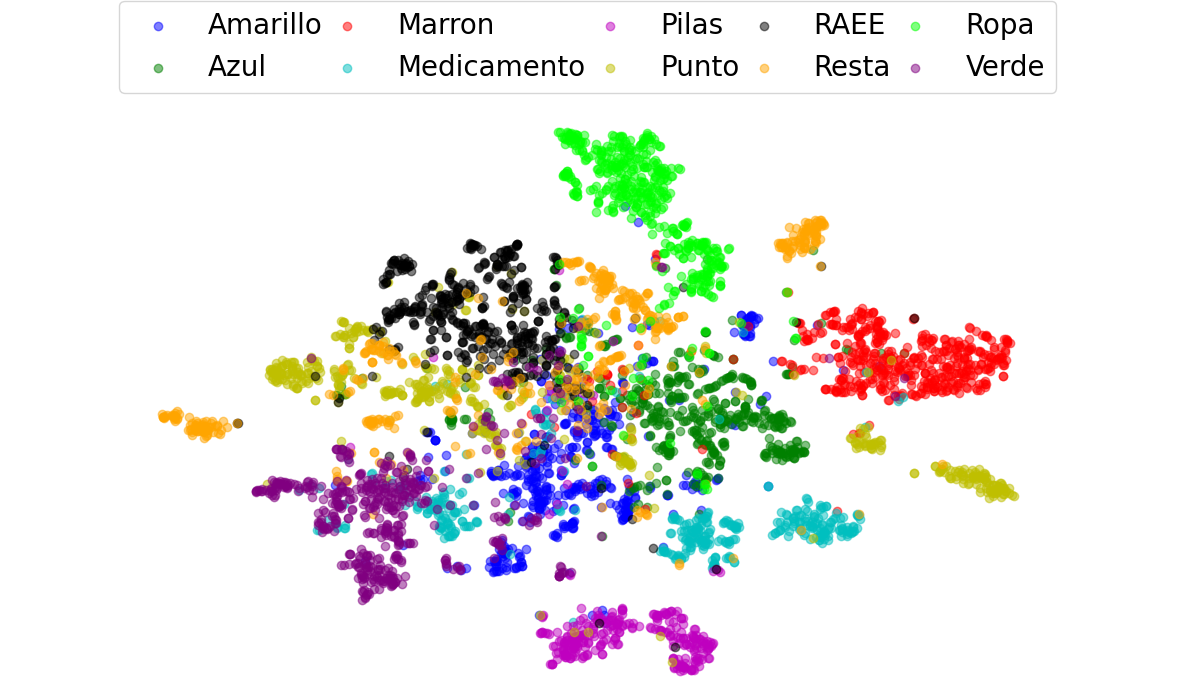
\includegraphics[width=1.0\textwidth]{img/distanciaclases.png}
    \caption{Visualización de los datos de validación en un espacio de 2 dimensiones generados por
    las características extraídas por el modelo Xception.}
  \end{subfigure}
  \centering
  \begin{subfigure}[b]{0.45\textwidth}
    \centering
    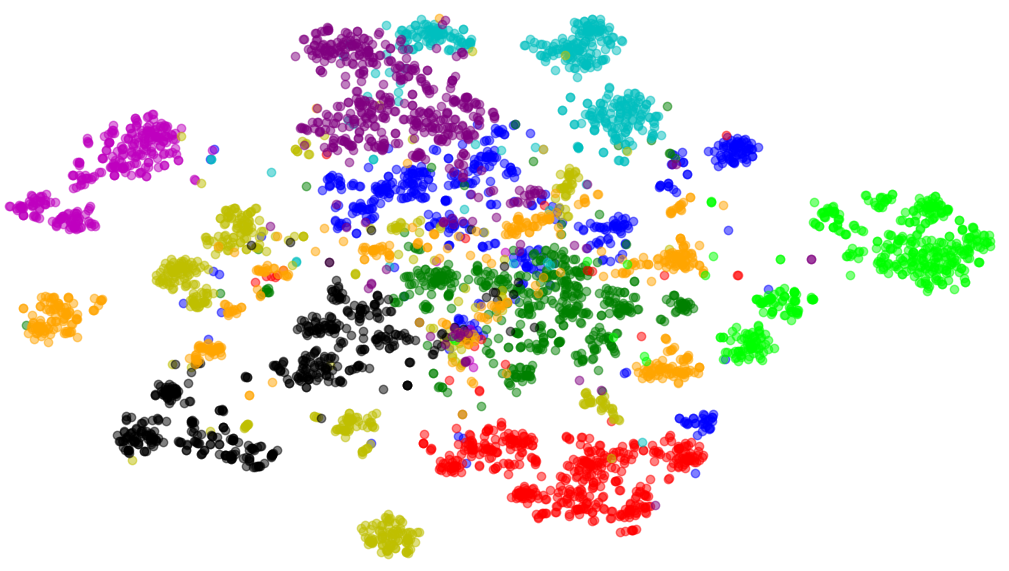
\includegraphics[width=0.8\textwidth]{img/clip_tsne.png}
    \caption{Visualización de los datos de validación en un espacio de 2 dimensiones generados por
    las características extraídas por el modelo OpenCLIP.}
  \end{subfigure}
  \caption{Comparativa de las visualizaciones de los datos de validación.}
  \label{fig:distanciaclases}
\end{figure}

Al observar los dos espacios de características en la Figura \ref{fig:distanciaclases}, el espacio
de características generado por OpenCLIP se ve mucho más separado que el generado por Xception. Esto
significa que las características extraídas por OpenCLIP son más discriminativas que las extraídas
por Xception por lo tanto el modelo lineal entrenado con estas características tendrá un mejor
rendimiento.

\begin{table*}[h]
  \centering
  \begin{tabular}{l|cccccccccc|c}
  \toprule
                        & Amarillo & Azul & Marron & Medica & Pilas & Punto & RAEE & Resta & Ropa & Verde & Mean acc     \\
  \midrule
  Xception              & 0.88     & 0.85 & 0.96   & 0.9    & 0.98  & 0.86  & 0.91 & 0.87 & 0.96 & 0.89  & 0.9            \\
  mobilenetV2           & 0.9      & 0.84 & 0.97   & 0.83   & 0.97  & 0.81  & 0.86 & 0.84 & 0.94 & 0.87  & 0.88           \\
  \midrule
  Zero Shot OpenCLIP    & 0.79     & 0.67 & 0.76   & 0.67   & 0.94  & 0.82  & 0.95 & 0.64 & 0.8  & 0.78  & 0.78           \\
  Linear-probe OpenCLIP & \textbf{0.92} & \textbf{0.91} & \textbf{0.97} & \textbf{0.9} & \textbf{0.99} & \textbf{0.89} & \textbf{0.95} & \textbf{0.88} & \textbf{0.99} & \textbf{0.9} & \textbf{0.93} \\
  \bottomrule
  \end{tabular}
  \caption{Comparativa de los modelos con los datos de validación.}
  \label{tab:my_label}
\end{table*}

Si comparamos los resultados de los modelos con los datos de validación, ver Tabla \ref{tab:my_label},
podemos observar que el modelo Linear-probe OpenCLIP es el que mejor rendimiento
tiene con una precisión de 0.93 en los datos de validación.

\begin{figure}[h]
  \centering
  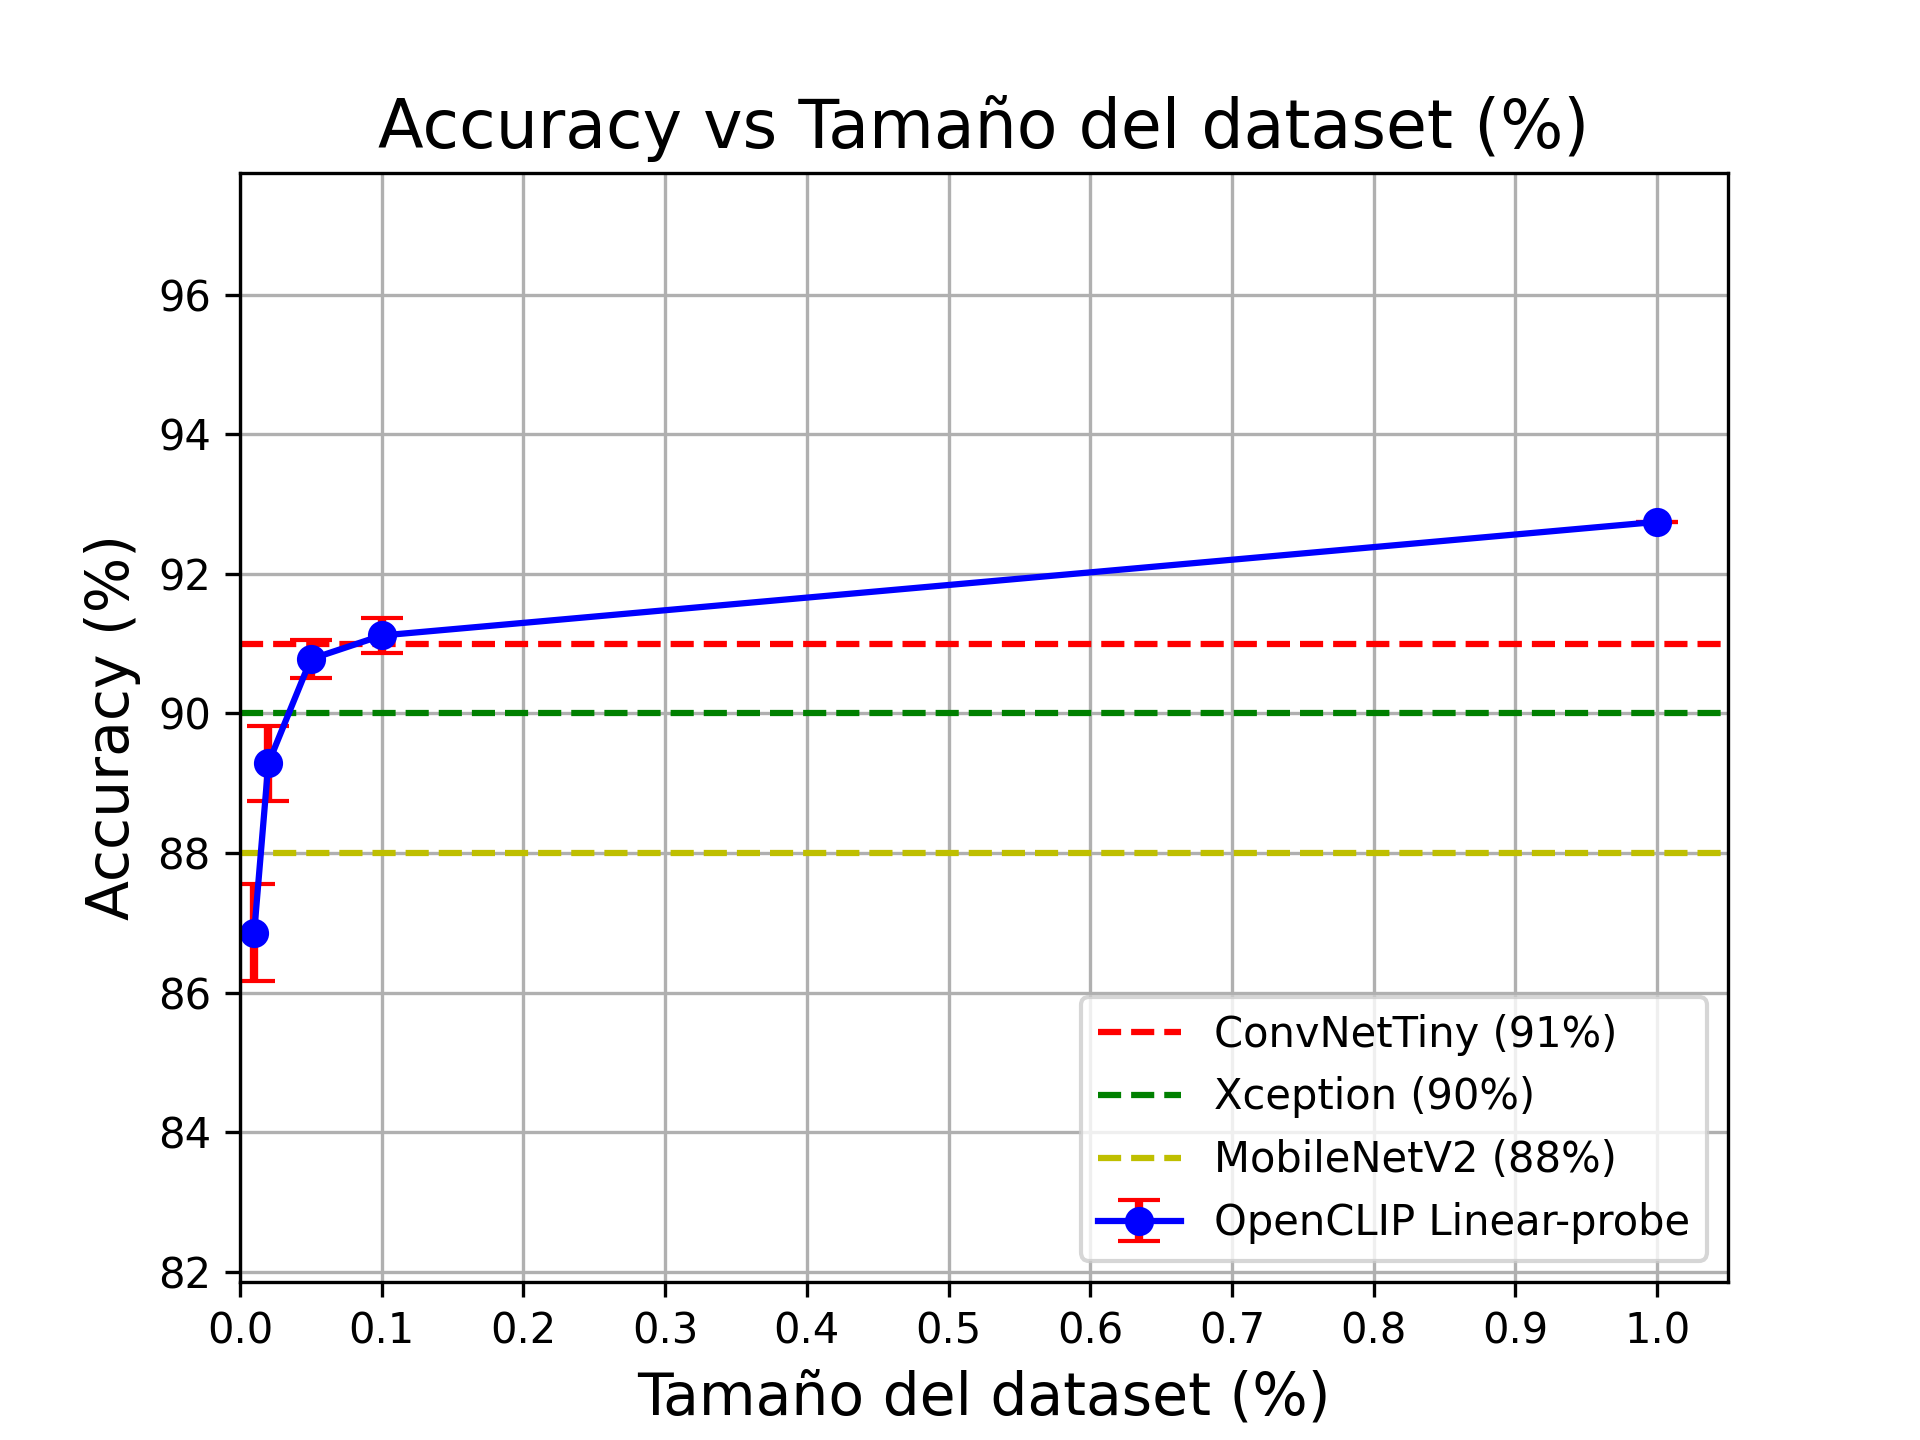
\includegraphics[width=0.50\textwidth]{img/accuracy_vs_percentile.png}
  \caption{Accuracy en función del numero de imágenes de entrenamiento.}
  \label{fig:accuracy_vs_percentile}
\end{figure}

Al ver el buen resultado del OpenCLIP, se ha decidido comprobar como se comporta si reducimos los datos de entrenamiento.

Lo que es interesante de la Figura \ref{fig:accuracy_vs_percentile} es que muestra que el modelo Linear-probe OpenCLIP es capaz de obtener una precisión del 91\% con tan solo el 10\% del conjunto de datos de entrenamiento. Este es un resultado impresionante y muestra la eficiencia de este modelo. En la mayoría de los casos, necesitamos un gran volumen de datos para entrenar un modelo de aprendizaje automático para que sea efectivo, pero el Linear-probe OpenCLIP parece ser capaz de ``aprender'' mucho de un conjunto de datos más pequeño.

Esto contrasta con los modelos Xception y MobilenetV2, que pueden no haber obtenido resultados tan buenos.

\begin{table*}[h]
  \centering % Centers the table
  \begin{tabular}{@{}l|cccccccccc|c@{}} % Makes the table fit within the page margin
  \toprule % Top horizontal line
  & Amarillo & Azul & Marron & Medica & Pilas & Punto & RAEE & Resta & Ropa & Verde & Mean Acc \\
  \midrule % Middle horizontal line
  Aire & 0.15 & 0.10 & 0.40 & 0.00 & 0.10 & 0.30 & 0.00 & 0.00 & 0.00 & 0.00 & 0.10 \\
  Aire + Material & 0.75 & 0.30 & 0.40 & 0.00 & 0.10 & 0.30 & 0.00 & 0.00 & 0.00 & 0.80 & 0.27 \\
  \midrule
  Xception & 0.57 & 0.44 & 0.89 & 0.47 & 0.75 & 0.52 & 0.90 & 0.41 & \textbf{0.90} & 0.80 & 0.67 \\
  MobileNetV2 & 0.67 & 0.39 & 0.84 & 0.06 & 0.60 & 0.48 & 0.85 & 0.55 & 0.80 & 0.75 & 0.60 \\
  \midrule
  OpenCLIP Zero-Shot & \textbf{1.00} & \textbf{0.55} & 0.79 & \textbf{0.82} & 0.90 & \textbf{1.00} & \textbf{0.95} & \textbf{0.91} & 0.85 & \textbf{0.95} & \textbf{0.87} \\
  OpenCLIP Linear-probe & 0.90 & \textbf{0.55} & \textbf{0.95} & 0.60 & \textbf{0.95} & 0.60 & 0.70 & 0.60 & 0.75 & 0.80 & 0.73 \\
  \bottomrule % Bottom horizontal line
  \end{tabular}
  \caption{Comparativa de los modelos desarrollados con la aplicación Aire con un dataset de Test. Por cada clase tenemos la siguiente cantidad de imágenes: Amarillo (21), Azul (18), Marrón (19), Medica (17), Pilas (20), Punto (21), RAEE (20), Resta (22), Ropa (20), Verde (20).}
  \label{table:comparativa_aire}

\end{table*}

Finalmente, en la Tabla \ref{table:comparativa_aire}, se ha analizado y comparado la eficacia de varias técnicas de clasificación de residuos, incluyendo la aplicación Aire, junto con varios modelos de aprendizaje profundo como Xception, MobileNetV2, OpenCLIP Zero-Shot y OpenCLIP Linear-probe. Los modelos se han comparado en base a su precisión media en la clasificación de diferentes tipos de residuos: Amarillo, Azul, Marrón, Médica, Pilas, Punto, RAEE, Resta, Ropa y Verde.

La versión base de la aplicación Aire mostró un rendimiento considerablemente más bajo en comparación con los otros modelos, con una precisión media de sólo el 10\%. Sin embargo, cuando se le añadió información adicional sobre los materiales (Aire + Material), indicandolelo mediante el chat, la precisión media aumentó al 27\%, demostrando una mejora significativa pero aún insuficiente frente a los modelos de aprendizaje profundo.

El modelo Xception, mostró un rendimiento decente, alcanzando una precisión media de 67\%. Por otro lado, MobileNetV2, también demostró un decente desempeño con una precisión media del 60\%.

Los modelos OpenCLIP, superaron a todos los demás modelos. En particular, el modelo OpenCLIP Zero-Shot demostró una precisión asombrosa en la clasificación de residuos, alcanzando una precisión media de 87\%. El modelo OpenCLIP Linear-probe también mostró un buen desempeño con una precisión media del 73\%.

Estos resultados sugieren que los enfoques basados en aprendizaje profundo zero-shot, pueden ofrecer mejoras sustanciales en la clasificación de residuos en comparación con las soluciones basadas en aplicaciones como Aire.

Por lo tanto, estos hallazgos apoyan la implementación y el uso de técnicas de aprendizaje profundo en la clasificación de residuos para lograr una mayor precisión y eficiencia en esta tarea crítica.

\subsection{Imágenes similares}

Para mejorar la eficacia del sistema de clasificación de imágenes y ayudar al usuario cuando el modelo de clasificación se encuentre en una situación de incertidumbre, se ha implementado un algoritmo de búsqueda de imágenes similares. Este algoritmo, dada una imagen proporcionada por el usuario, devuelve las tres imágenes más parecidas a la imagen de entrada.

El proceso se puede dividir en dos fases esenciales: la extracción de características de la imagen y la búsqueda de imágenes similares.

Para la extracción de características, se ha utilizado por el buen desempleño OpenCLIP. La imagen de entrada tiene una forma de $224 \times 224 \times 3$ (ancho, alto y canales de color respectivamente), y luego se transforma a un vector de características de 1024 dimensiones a través del encoder visual de OpenCLIP.

Una vez obtenido el vector de características, este se utiliza como entrada para un algoritmo de K Nearest Neighbors (KNN). El KNN se encarga de calcular la distancia euclídea entre la representación vectorial de la imagen de entrada y las representaciones de todas las imágenes en el dataset.

Después de calcular estas distancias (distancia del coseno), el algoritmo KNN devuelve las tres imágenes cuyos vectores de características son los más cercanos al vector de características de la imagen de entrada. En otras palabras, devuelve las tres imágenes más similares a la imagen proporcionada por el usuario.

\begin{figure}[h]
  \centering
  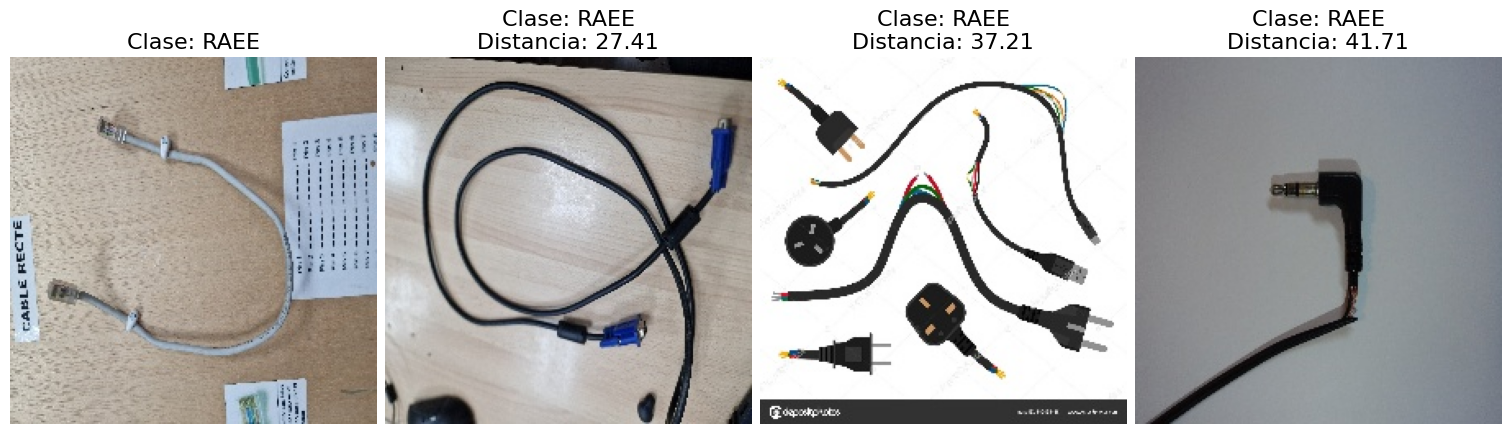
\includegraphics[width=0.50\textwidth]{img/sim_raee.png}
  \caption{Visualización de imágenes similares de los datos de validación con imágenes de entrenamiento. La primera imagen es la imagen de entrada, y las tres siguientes son las imágenes más similares.}
  \label{fig:sim_raee}
\end{figure}

Este enfoque proporciona una capa adicional de flexibilidad al sistema de clasificación, permitiendo al usuario seleccionar la etiqueta más adecuada, como se puede observar en la Figura \ref{fig:sim_raee}. En este caso, el usuario ha proporcionado una imagen de un cable (RAEE), y ha devuelto tres imágenes similares de cables, El usuario puede entonces seleccionar la etiqueta más adecuada para la imagen de entrada en caso de no estar de acuerdo con la predicción del modelo de clasificación.

\section{Arquitectura de la Aplicación}

Para ofrecer la funcionalidad de detección de objetos en imágenes y sugerir imágenes similares desde la base de datos, se ha desarrollado una API utilizando FastAPI. La API presenta un endpoint, ``/process\_image'', que se encarga de recibir una imagen, procesarla y devolver la información relevante para su visualización en la aplicación. La arquitectura de este sistema se ilustra en la Figura \ref{fig:arquitectura}.

\begin{figure*}[h]
\centering
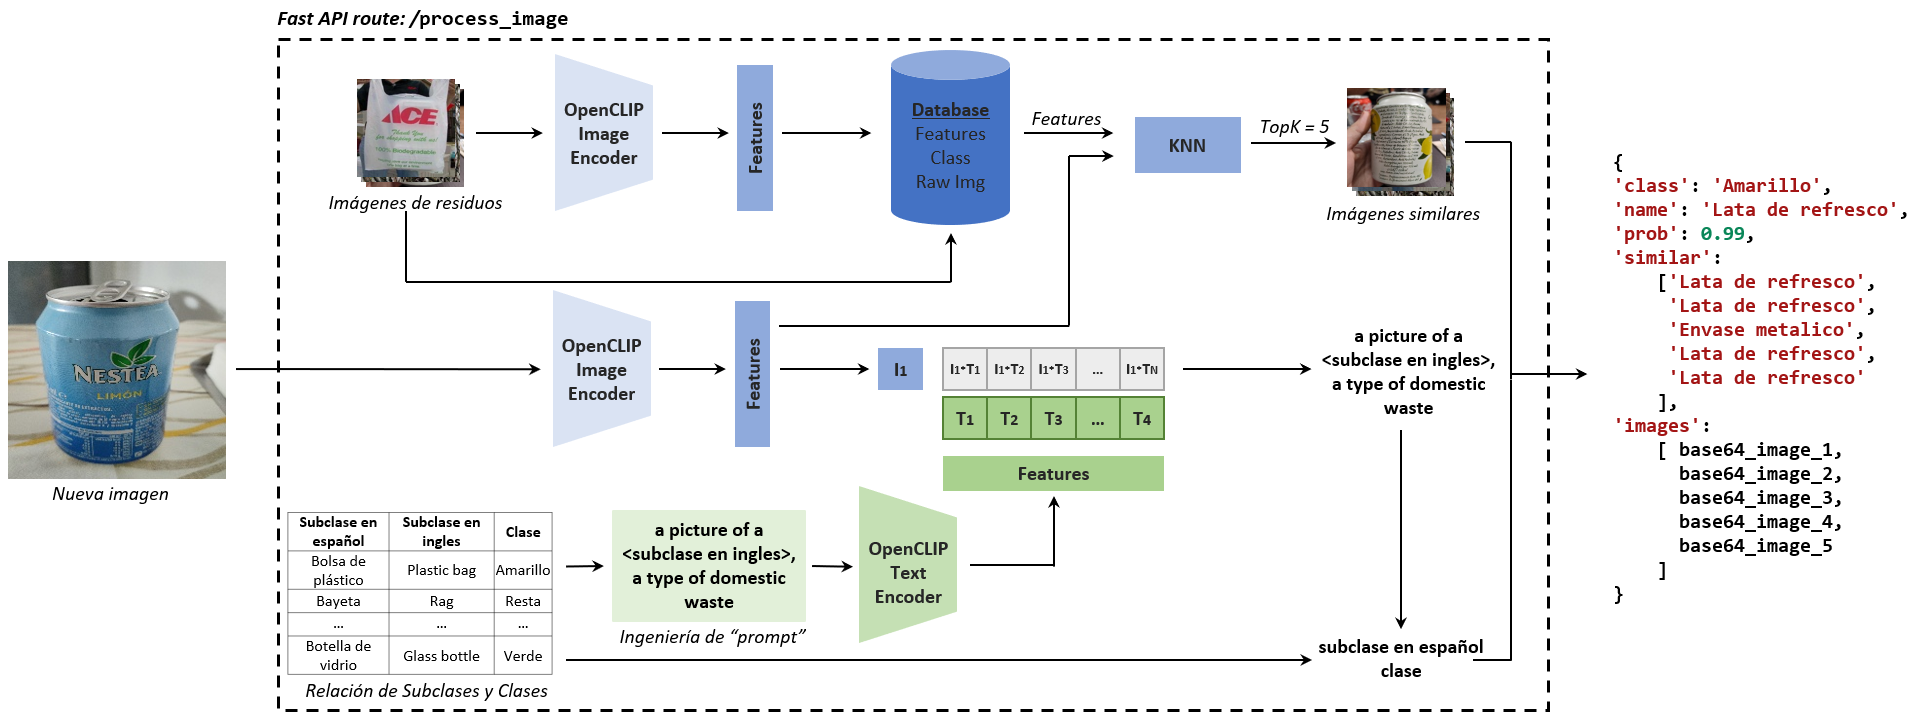
\includegraphics[width=1.0\textwidth]{img/Arquitectura1.png}
\caption{Arquitectura del despliegue del modelo de clasificación OpenCLIP para la clasificación de residuos.}
\label{fig:arquitectura}
\end{figure*}

Inicialmente, se extraen las características de todas las imágenes en el conjunto de datos de la base de datos. Esta información se guarda en un archivo que también registra la clase del objeto, la dirección de la imagen original y las características extraídas.

Cuando se hace una solicitud a ``/process\_image'' con una nueva imagen, la API ejecuta un proceso de dos pasos. Primero, extrae las características de la imagen. Con estas características, realiza una búsqueda de las cinco imágenes más similares a la imagen recibida utilizando el algoritmo k-nearest neighbors (KNN) con la distancia del coseno. Simultáneamente, emplea las características extraídas para clasificar la imagen. Este proceso de clasificación se basa en los prompts que se han creado específicamente para la clasificación de residuos.

Finalmente, toda esta información se devuelve en formato JSON para su uso en la aplicación.

Un diagrama detallado de los componentes y su interacción en el sistema se puede encontrar en los apéndices, en la Figura \ref{fig:diagrama_caso_uso}.

\section{Trabajo futuro}

En este trabajo se ha desarrollado una aplicación para clasificar residuos utilizando aprendizaje profundo. Sin embargo, hay muchas formas en las que se puede mejorar la aplicación para que sea más eficaz y útil. Entre
ellas se encuentran, la segmentación de objetos dentro de la misma imagen para poder separar los posibles materiales antes de tirar el residuo. Para ello se ha investigado
un poco de como se podría implementar y se han encontrado varias formas de hacerlo.

\subsection{Segmentación de objetos}

Unos de los principales problemas de utilizar clasificación en imágenes es que no se puede saber la localización de los objetos en la imagen. Para ello es necesario crear un dataset de segmentación, pero el coste en tiempo humano para etiquetar las imágenes es muy elevado.
Para solucionar este problema se ha buscado métodos de segmentación utilizando Segment Anything \cite{sammeta} de Meta para poder segmentar y clasificar las imágenes de la manera automática y terminar de etiquetar las imágenes que no se han podido etiquetar correctamente de manera manual.
Segment Anything funciona de dos maneras distintas, en la primera se le pasa una imagen y devuelve una imagen con los objetos segmentados, en la segunda se le pasa una imagen y puntos donde se encuentra el objeto y puntos que es el fondo y devuelve una mascara del objeto.

Sabiendo esto se puede afrontar el problema de clasificación automática de diversas formas.

\subsubsection{Clasificación de mascaras}

Este método consiste en usar Segment Anything en una imagen y que devuelva un listado de mascaras de todos los objetos que se encuentran en la imagen. Una vez se tiene este listado de mascaras se puede pasar a la red neuronal para que clasifique cada una de las imágenes nuevas.

\begin{figure}[h!]
  \centering
  \begin{subfigure}[b]{0.10\textwidth}
    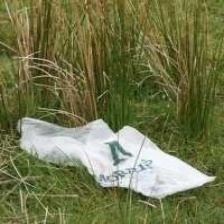
\includegraphics[width=\textwidth]{img/clasificacion/input.jpg}
    \caption{Entrada}
  \end{subfigure}
  \hfill
  \begin{subfigure}[b]{0.10\textwidth}
    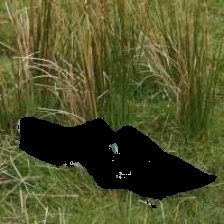
\includegraphics[width=\textwidth]{img/clasificacion/mask_0.jpg}
    \caption{Mascara 1}
  \end{subfigure}
  \hfill
  \begin{subfigure}[b]{0.10\textwidth}
    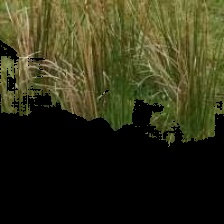
\includegraphics[width=\textwidth]{img/clasificacion/mask_1.jpg}
    \caption{Mascara 2}
  \end{subfigure}
  \hfill
  \begin{subfigure}[b]{0.10\textwidth}
    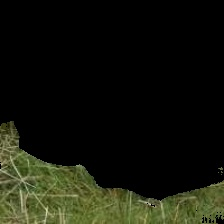
\includegraphics[width=\textwidth]{img/clasificacion/mask_2.jpg}
    \caption{Mascara 3}
  \end{subfigure}
  
  \vspace{10pt} % espacio vertical entre las dos filas
  
  \begin{subfigure}[b]{0.10\textwidth}
    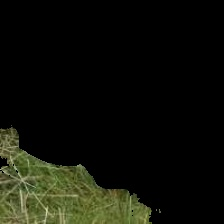
\includegraphics[width=\textwidth]{img/clasificacion/mask_3.jpg}
    \caption{Mascara 4}
  \end{subfigure}
  \hfill
  \begin{subfigure}[b]{0.10\textwidth}
    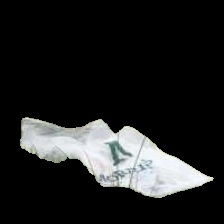
\includegraphics[width=\textwidth]{img/clasificacion/mask_4.jpg}
    \caption{Mascara 5}
  \end{subfigure}
  \hfill
  \begin{subfigure}[b]{0.10\textwidth}
    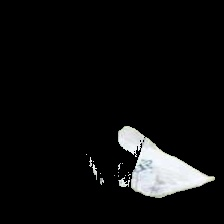
\includegraphics[width=\textwidth]{img/clasificacion/mask_5.jpg}
    \caption{Mascara 6}
  \end{subfigure}
  \hfill
  \begin{subfigure}[b]{0.10\textwidth}
    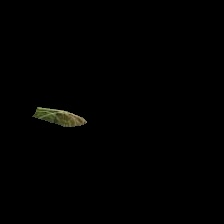
\includegraphics[width=\textwidth]{img/clasificacion/mask_6.jpg}
    \caption{Mascara 7}
  \end{subfigure}
  \caption{Imagen de entrada y mascaras de los objetos detectados. La mascara que el clasificador ha escogido ha sido la (g).}
  \label{fig:clasificacion_sam}
\end{figure}

Una vez tenemos las mascaras de los objetos se puede pasar a la red neuronal
para que clasifique cada una de las imágenes nuevas y nos quedamos con la clase que mayor
porcentaje de confianza tenga.

Este método tiene el problema de confundir objetos o zonas de la imagen que no nos interesa como si fuera el objeto que se esta clasificando como se indica en la Figura \ref{fig:clasificacion_sam}. Por lo que es necesario descartar aquellas mascaras que no se correspondan con el objeto que se esta clasificando, para ello
necesitamos poner un atención visual en la imagen para saber donde se encuentra el objeto que se esta clasificando.

\subsubsection{Atención visual para las mascaras}

Para seleccionar las macara idónea se puede utilizar la técnica de Salency map de esta manera podemos saber donde se encuentra el objeto que se esta clasificando y descartar las mascaras que no se encuentren en esa zona.

\begin{figure}[h!]
  \centering
  \begin{subfigure}[b]{0.115\textwidth}
    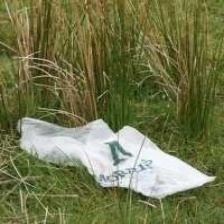
\includegraphics[width=\textwidth]{img/clasificacion/input.jpg}
    \caption{Entrada}
  \end{subfigure}
  \begin{subfigure}[b]{0.115\textwidth}
    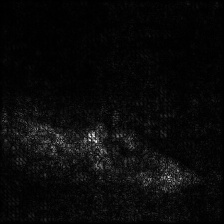
\includegraphics[width=\textwidth]{img/clasificacion/saliency_map_vanilla.jpg}
    \caption{Salency map}
  \end{subfigure}
  \begin{subfigure}[b]{0.115\textwidth}
    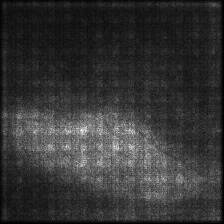
\includegraphics[width=\textwidth]{img/clasificacion/saliency_map.jpg}
    \caption{Smooth Grad}
  \end{subfigure}
  \begin{subfigure}[b]{0.115\textwidth}
    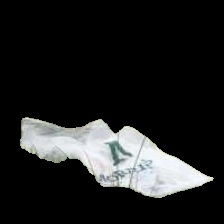
\includegraphics[width=\textwidth]{img/clasificacion/mask_4.jpg}
    \caption{Mascara}
  \end{subfigure}
  \caption{Comparativa de salency map y smooth grad para seleccionar la mascara idónea que maximiza los valores del SmoothGrad.}
\end{figure}

De esta manera podemos descartar las mascaras que no se encuentren en la zona de interés y quedarnos con las que si se encuentren en esa zona.

\subsubsection{Optimización de puntos de atención}

Este método utiliza técnicas de aprendizaje automático para identificar los ``puntos de atención'' más relevantes en una imagen, es decir,
las áreas que más contribuyen a la identificación de un objeto en particular. Primero se crea un ``mapa de activación'' para destacar estas áreas.
Luego, se aplica una máscara sobre estas áreas y se utiliza un modelo de clasificación para predecir qué objeto se encuentra allí. Finalmente,
se realiza una optimización para encontrar las mejores áreas a las que prestar atención, con el objetivo de mejorar la precisión
de la clasificación del objeto.

\subsubsection{Comparativa visual de los métodos}

Las pruebas se han realizado con 6 imágenes del dataset de entrenamiento escogidas aleatoriamente, mirar Tabla \ref{tab:metodos_sam}.

\begin{table}[ht]
  \centering
  \begin{tabularx}{0.5\textwidth}{XXXX}
  \centering
  \textbf{Imagen} & \textbf{Clasificación} & \centering\textbf{Salency} & \textbf{Optimización} \\
  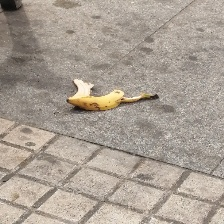
\includegraphics[width=\linewidth]{img/clasificacion/img0.jpg} & 
\includegraphics[width=\linewidth]{img/clasificacion/img0_p.jpg}  & 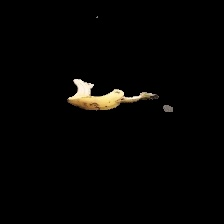
\includegraphics[width=\linewidth]{img/clasificacion/img0_s.jpg} & 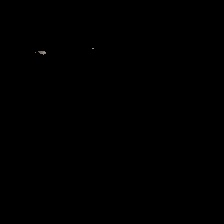
\includegraphics[width=\linewidth]{img/clasificacion/img0_o.jpg} \\
  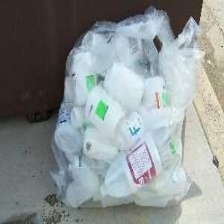
\includegraphics[width=\linewidth]{img/clasificacion/img1.jpg} & 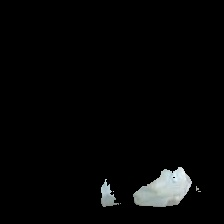
\includegraphics[width=\linewidth]{img/clasificacion/img1_p.jpg}  & 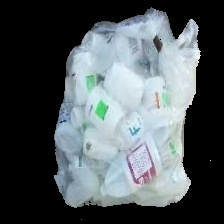
\includegraphics[width=\linewidth]{img/clasificacion/img1_s.jpg} & 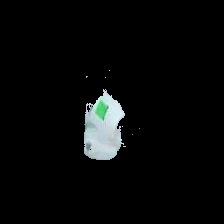
\includegraphics[width=\linewidth]{img/clasificacion/img1_o.jpg} \\
  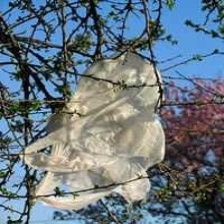
\includegraphics[width=\linewidth]{img/clasificacion/img2.jpg} & 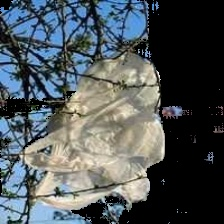
\includegraphics[width=\linewidth]{img/clasificacion/img2_p.jpg}  & 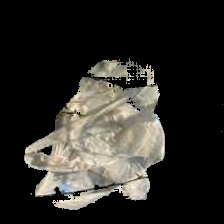
\includegraphics[width=\linewidth]{img/clasificacion/img2_s.jpg} & 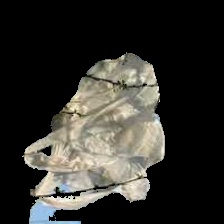
\includegraphics[width=\linewidth]{img/clasificacion/img2_o.jpg} \\
  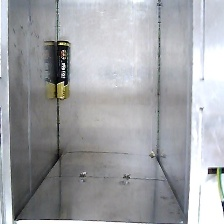
\includegraphics[width=\linewidth]{img/clasificacion/img3.jpg} & 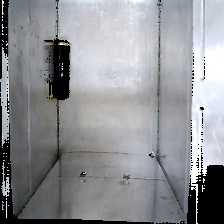
\includegraphics[width=\linewidth]{img/clasificacion/img3_p.jpg}  & 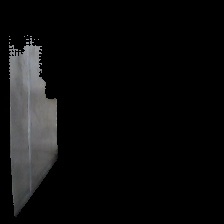
\includegraphics[width=\linewidth]{img/clasificacion/img3_s.jpg} & 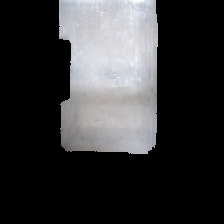
\includegraphics[width=\linewidth]{img/clasificacion/img3_o.jpg} \\
  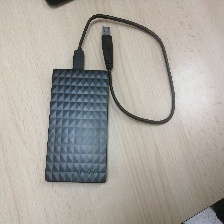
\includegraphics[width=\linewidth]{img/clasificacion/img6.jpg} & 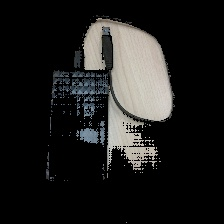
\includegraphics[width=\linewidth]{img/clasificacion/img6_p.jpg}  & 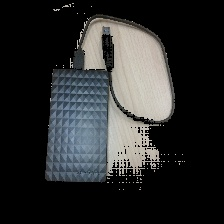
\includegraphics[width=\linewidth]{img/clasificacion/img6_s.jpg} & 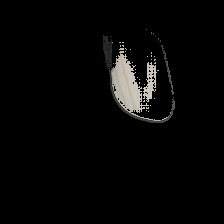
\includegraphics[width=\linewidth]{img/clasificacion/img6_o.jpg} \\
\end{tabularx}
  \caption{Comparativa visual de las distintas técnicas para generar mascaras del objeto. En la primera columna tenemos la imagen original, en la segunda el método de clasificación de mascara, en la tercera método de Salency Map y en la cuarta el método de optimización de puntos.}
  \label{tab:metodos_sam}
\end{table}

Como resultado se ha obtenido que el método de Salency Map es el más robusto.

\section{Conclusiones}

En base a los objetivos planteados y los resultados obtenidos en este estudio, puedo concluir lo siguiente:

Primero, se ha logrado generar un dataset, compuesto por más de 48000 imágenes, para cubrir una amplia gama de residuos reciclables y no reciclables. Este logro fue posible, en parte, mediante el uso de una aplicación móvil para permitir un etiquetado colaborativo, ampliando considerablemente la diversidad y cantidad de los datos recolectados.

Segundo, se ha desarrollado una aplicación móvil capaz de superar a las aplicaciones existentes en la clasificación automatizada de residuos. En comparación con Aire, la única otra aplicación a nivel nacional doméstica que acepta imágenes, mi aplicación demostró una superioridad significativa. Esta mejora facilitará el proceso de reciclaje para los usuarios, permitiéndoles clasificar de manera más eficiente sus residuos.

Tercero, he explorado la viabilidad de generar un conjunto de datos semánticos a partir de uno de clasificación y se ha demostrado que es posible segmentar las imágenes en base a su etiqueta de clasificación pero que aun así se necesita un etiquetado manual para mejorar la calidad de las segmentaciones en algunas imágenes.

Por último, en cuanto a las técnicas de aprendizaje automático, encontramos que OpenCLIP proporcionó los mejores resultados en las tareas. En particular, ha demostrado ser altamente efectivo en tareas de zero-shot, lo que permite la clasificación de objetos que no se encuentran en el conjunto de datos de entrenamiento. Esto es especialmente útil para la clasificación de residuos, ya que los residuos reciclables pueden variar mucho de una región a otra o
incluso en la misma región con el tiempo.

% Agradecimientos
\section*{Agradecimientos}

Quiero agradecer sobretodo a mi tutor, Coen Antens, por dejarme total libertad durante el desarrollo de este proyecto.
También quiero agradecer a todos aquellos que han participado en el etiquetado de las imágenes, en especial mis alumnos que son los que más han participado
durante el etiquetado con la aplicación móvil.

\begin{thebibliography}{11}

\bibitem{reciclaje}
Por que es importante reciclar https://ecoembesdudasreciclaje.es/por-que-es-importante-reciclar/

\bibitem{green-deal}
Green Deal https://commission.europa.eu/strategy\-and\-policy/priorities\-2019\-2024/european\-green\-deal\_es

\bibitem{transformers}
Vaswani, A., Shazeer, N., Parmar, N., Uszkoreit, J., Jones, L., Gomez, A. N., … Polosukhin, I. (2017). Attention Is All You Need. doi:10.48550/ARXIV.1706.03762

\bibitem{clip}
Radford, A., Kim, J. W., Hallacy, C., Ramesh, A., Goh, G., Agarwal, S., … Sutskever, I. (2021). Learning Transferable Visual Models From Natural Language Supervision. doi:10.48550/ARXIV.2103.00020

\bibitem{chollet2017xception}
Chollet, F. (2017). Xception: Deep Learning with Depthwise Separable Convolutions. In Proceedings of the IEEE Conference on Computer Vision and Pattern Recognition (pp. 1800-1807). https://doi.org/10.1109/CVPR.2017.195

\bibitem{he2016identity}
He, K., Zhang, X., Ren, S., \& Sun, J. (2016). Identity Mappings in Deep Residual Networks. arXiv preprint arXiv:1603.05027.

\bibitem{huang2018densely}
Huang, G., Liu, Z., Van Der Maaten, L., \& Weinberger, K. Q. (2018). Densely connected convolutional networks. In Proceedings of the IEEE conference on computer vision and pattern recognition (pp. 4700-4708).

\bibitem{howard2019searching}
Howard, A., Sandler, M., Chu, G., Chen, L. C., Chen, B., Tan, M., ... Adam, H. (2019). Searching for MobileNetV3. arXiv preprint arXiv:1905.02244.

\bibitem{sandler2018mobilenetv2}
Sandler, M., Howard, A., Zhu, M., Zhmoginov, A., \& Chen, L. (2019). MobileNetV2: Inverted Residuals and Linear Bottlenecks. arXiv preprint arXiv:1801.04381.

\bibitem{szegedy2016rethinking}
Szegedy, C., Vanhoucke, V., Ioffe, S., Shlens, J., \& Wojna, Z. (2015). Rethinking the Inception Architecture for Computer Vision. arXiv preprint arXiv:1512.00567.

\bibitem{szegedy2017inception}
Szegedy, C., Ioffe, S., Vanhoucke, V., \& Alemi, A. A. (2017). Inception-v4, Inception-ResNet and the Impact of Residual Connections on Learning. In Thirty-First AAAI Conference on Artificial Intelligence.

\bibitem{Liu2020conv}
Liu, Z., Mao, H., Wu, C.-Y., Feichtenhofer, C., Darrell, T., \& Xie, S. (2022). A ConvNet for the 2020s. arXiv preprint arXiv:2201.03545.

\bibitem{Zoph2018}
Zoph, B., Vasudevan, V., Shlens, J., \& Le, Q. V. (2018). Learning Transferable Architectures for Scalable Image Recognition. arXiv preprint arXiv:1707.07012.

\bibitem{vgg16}
Simonyan, K., \& Zisserman, A. (2015). Very Deep Convolutional Networks for Large-Scale Image Recognition. arXiv preprint arXiv:1409.1556.

\bibitem{sammeta}
Kirillov, A., Mintun, E., Ravi, N., Mao, H., Rolland, C., Gustafson, L., ... Girshick, R. (2023). Segment Anything. arXiv preprint arXiv:2304.02643.

\bibitem{hog}
N. Dalal and B. Triggs, "Histograms of oriented gradients for human detection," 2005 IEEE Computer Society Conference on Computer Vision and Pattern Recognition (CVPR'05), San Diego, CA, USA, 2005, pp. 886-893 vol. 1, doi: 10.1109/CVPR.2005.177.

\bibitem{SIFT}
Lowe, D. G. (2004). Distinctive Image Features from Scale-Invariant Keypoints. International Journal of Computer Vision, 60(2), 91–110. https://doi.org/10.1023/B:VISI.0000029664.99615.94

\bibitem{SURF}
Bay, H., Ess, A., Tuytelaars, T., \& Van Gool, L. (2008). Speeded-Up Robust Features (SURF). Computer Vision and Image Understanding, 110(3), 346–359. https://doi.org/10.1016/j.cviu.2007.09.014

\bibitem{svm}
Cortes, C., \& Vapnik, V. (1995). Support-vector networks. Machine Learning, 20(3), 273–297. https://doi.org/10.1007/BF00994018

\bibitem{random_forest}
Breiman, L. (2001). Random Forests. Machine Learning, 45(1), 5–32. https://doi.org/10.1023/A:1010933404324

\bibitem{lenet}
LeCun, Y., Bottou, L., Bengio, Y., \& Haffner, P. (1998). Gradient-Based Learning Applied to Document Recognition. Proceedings of the IEEE, 86(11), 2278–2324. https://doi.org/10.1109/5.726791

\bibitem{alexnet}
Krizhevsky, A., Sutskever, I., \& Hinton, G. E. (2012). ImageNet Classification with Deep Convolutional Neural Networks. In F. Pereira, C. J. C. Burges, L. Bottou, \& K. Q. Weinberger (Eds.), Advances in Neural Information Processing Systems 25 (pp. 1097–1105). Curran Associates, Inc.

\bibitem{vgg}
Simonyan, K., \& Zisserman, A. (2015). Very Deep Convolutional Networks for Large-Scale Image Recognition. arXiv preprint arXiv:1409.1556.

\bibitem{resnet}
He, K., Zhang, X., Ren, S., \& Sun, J. (2016). Deep Residual Learning for Image Recognition. In 2016 IEEE Conference on Computer Vision and Pattern Recognition (CVPR) (pp. 770–778). IEEE. https://doi.org/10.1109/CVPR.2016.90

\bibitem{grad_cam}
Selvaraju, R. R., Cogswell, M., Das, A., Vedantam, R., Parikh, D., \& Batra, D. (2017). Grad-CAM: Visual Explanations from Deep Networks via Gradient-Based Localization. In 2017 IEEE International Conference on Computer Vision (ICCV) (pp. 618–626). IEEE. https://doi.org/10.1109/ICCV.2017.74

\bibitem{ScoreCAM}
Wang, F., Jiang, M., Qian, C., Yang, S., Li, C., Zhang, H., Wang, X., \& Tang, X. (2020). Score-CAM: Score-Weighted Visual Explanations for Convolutional Neural Networks. In 2020 European Conference on Computer Vision (ECCV) (pp. 20–36). Springer International Publishing. https://doi.org/10.1007/978-3-030-58536-5\_2

\bibitem{LayerCAM}
Zhou, B., Khosla, A., Lapedriza, A., Oliva, A., \& Torralba, A. (2016). Learning Deep Features for Discriminative Localization. In 2016 IEEE Conference on Computer Vision and Pattern Recognition (CVPR) (pp. 2921–2929). IEEE. https://doi.org/10.1109/CVPR.2016.319

\bibitem{SalencyMap}
Simonyan, K., Vedaldi, A., \& Zisserman, A. (2013). Deep Inside Convolutional Networks: Visualising Image Classification Models and Saliency Maps. arXiv preprint arXiv:1312.6034.

\bibitem{SmoothGrad}
Smilkov, D., Thorat, N., Kim, B., Viégas, F., \& Wattenberg, M. (2017). SmoothGrad: removing noise by adding noise. arXiv preprint arXiv:1706.03825.

\bibitem{unet}
Ronneberger, O., Fischer, P., \& Brox, T. (2015). U-Net: Convolutional Networks for Biomedical Image Segmentation. In N. Navab, J. Hornegger, W. M. Wells, \& A. F. Frangi (Eds.), Medical Image Computing and Computer-Assisted Intervention – MICCAI 2015 (pp. 234–241). Springer International Publishing. https://doi.org/10.1007/978-3-319-24574-4\_28

\bibitem{deeplab}
Chen, L.-C., Papandreou, G., Kokkinos, I., Murphy, K., \& Yuille, A. L. (2018). DeepLab: Semantic Image Segmentation with Deep Convolutional Nets, Atrous Convolution, and Fully Connected CRFs. IEEE Transactions on Pattern Analysis and Machine Intelligence, 40(4), 834–848. https://doi.org/10.1109/TPAMI.2017.2699184

\bibitem{maskrcnn}
He, K., Gkioxari, G., Dollár, P., \& Girshick, R. (2017). Mask R-CNN. In 2017 IEEE International Conference on Computer Vision (ICCV) (pp. 2980–2988). IEEE. https://doi.org/10.1109/ICCV.2017.322

\bibitem{t-sne}
Maaten, L. van der, \& Hinton, G. (2008). Visualizing Data using t-SNE. Journal of Machine Learning Research, 9(Nov), 2579–2605.

\end{thebibliography}

\onecolumn

\appendix

\section*{Apéndice}

\setcounter{section}{1}

\subsection{Aplicación móvil}

\begin{figure}[h]
  \centering
  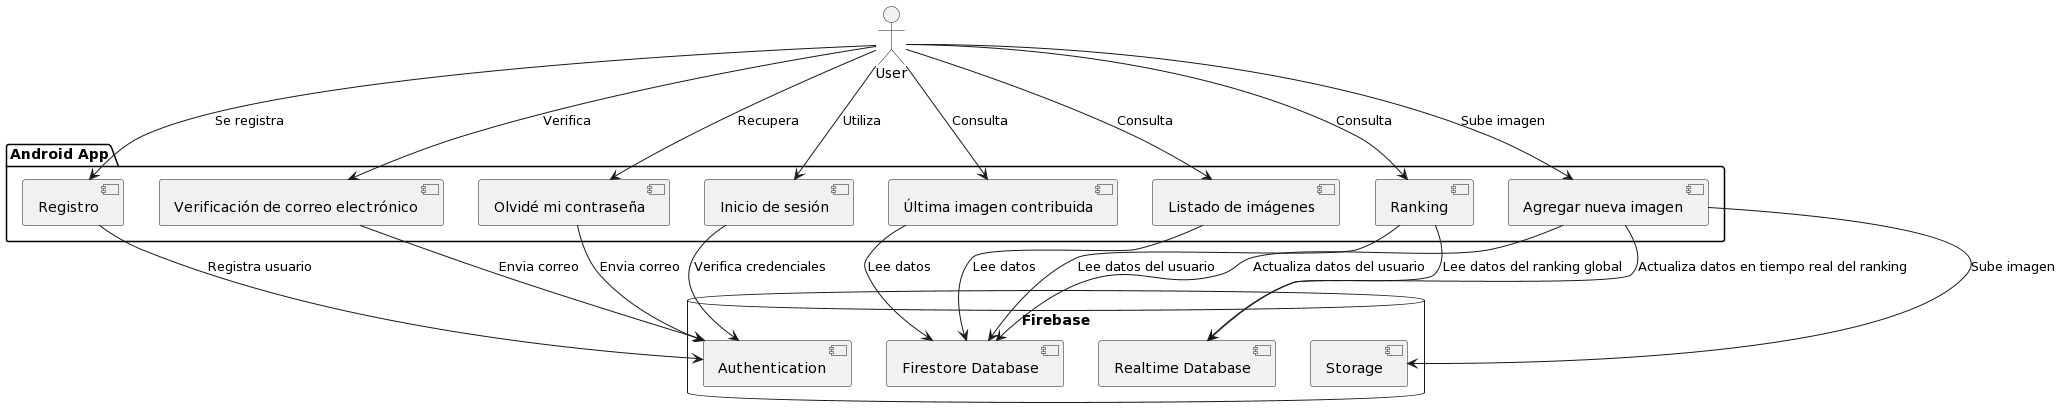
\includegraphics[width=0.95\textwidth]{img/diagrama_caso_uso.png}
  \caption{Diagrama de componentes de la aplicación Android para contribuir y visualizar imágenes en tiempo real utilizando Firebase como backend.}
  \label{fig:diagrama_caso_uso}
\end{figure}

\begin{figure}[h]
  \centering
  \begin{subfigure}[b]{0.16\textwidth}
    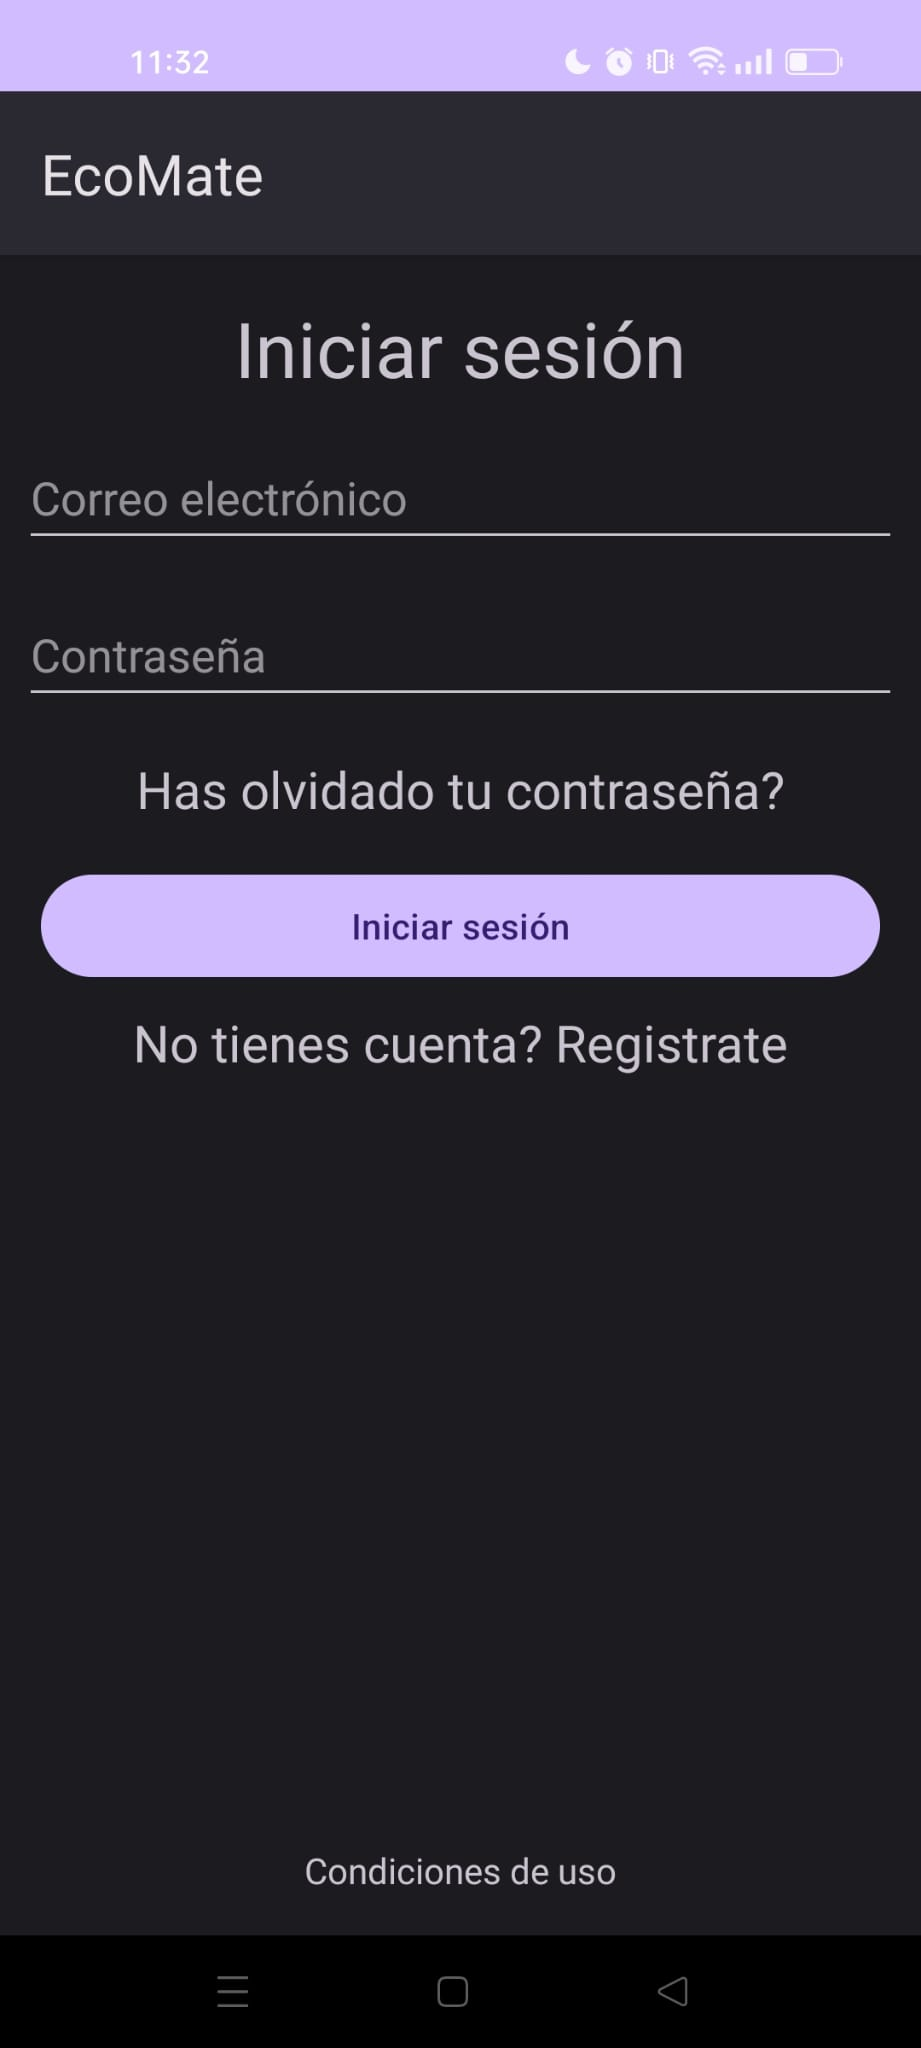
\includegraphics[width=\textwidth]{img/app_login.jpeg}
    \caption{Inicio de sesión}
    \label{fig:imagen1}
  \end{subfigure}
  \begin{subfigure}[b]{0.16\textwidth}
    
\includegraphics[width=\textwidth]{img/app_registro.jpeg}
    \caption{Registro}
    \label{fig:imagen2}
  \end{subfigure}
  \begin{subfigure}[b]{0.16\textwidth}
    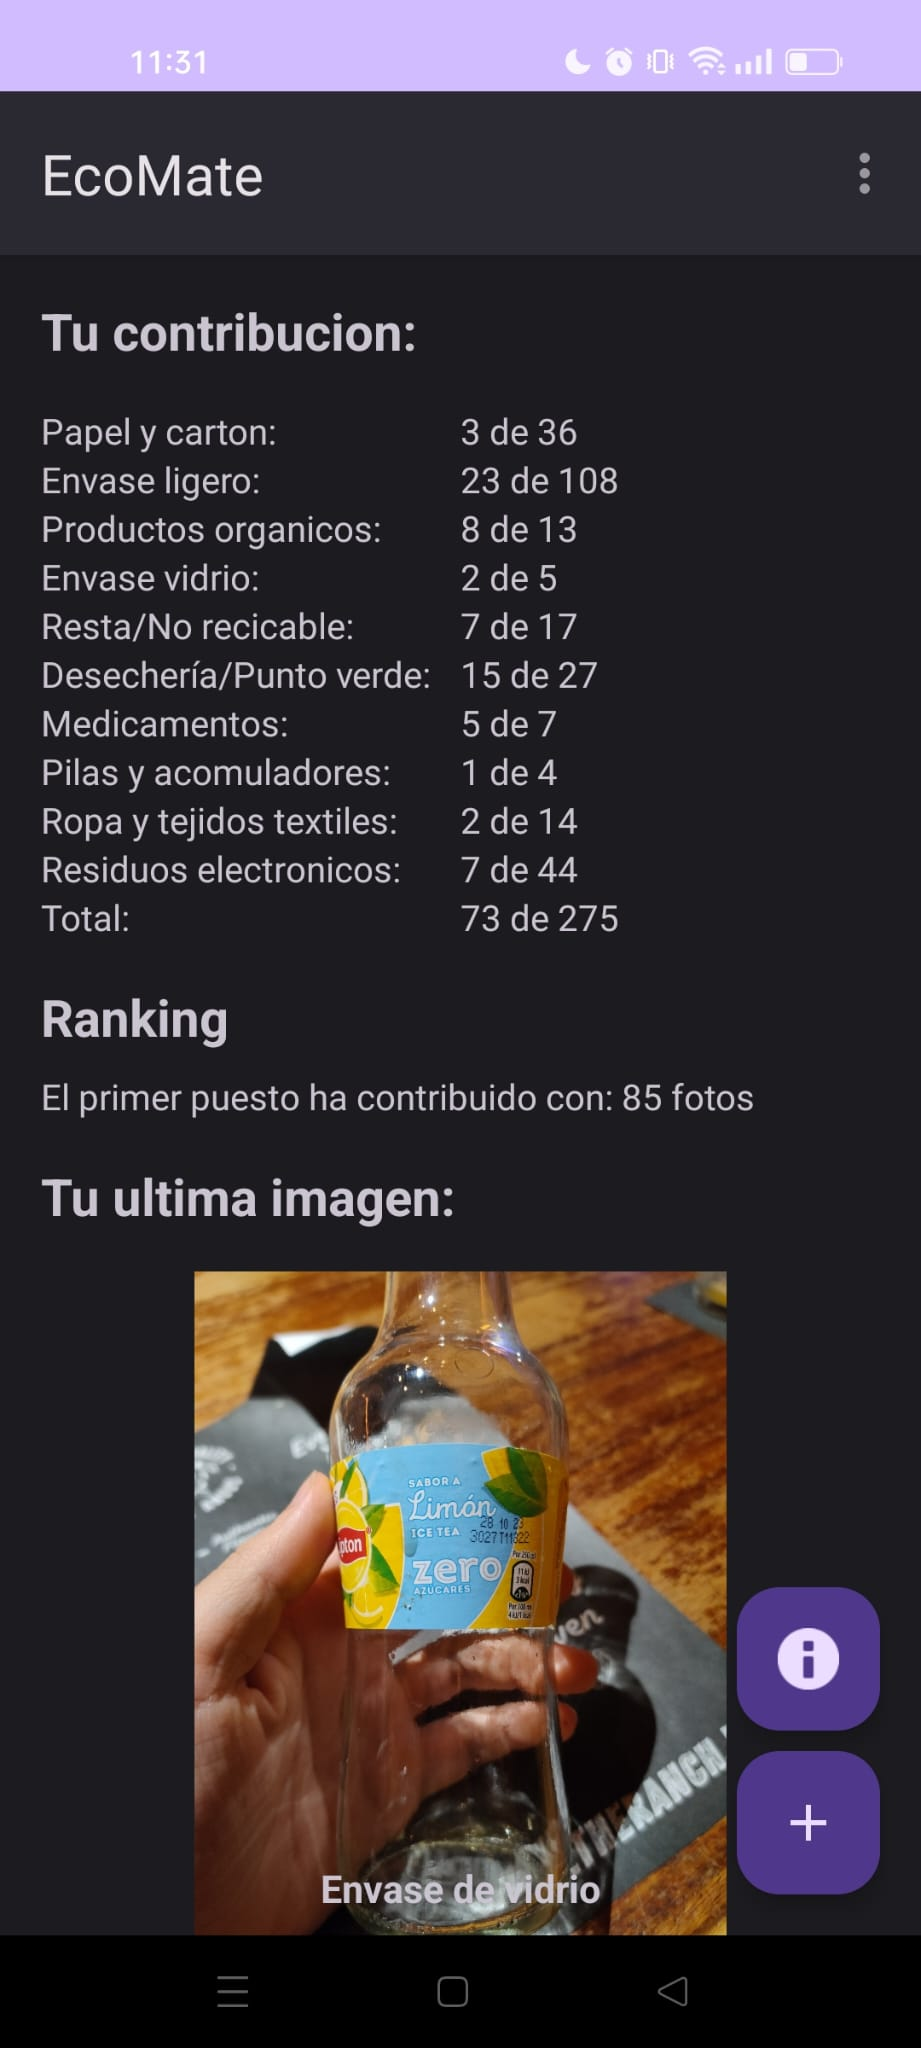
\includegraphics[width=\textwidth]{img/app_menu.jpeg}
    \caption{Menú principal}
    \label{fig:imagen3}
  \end{subfigure}
  \begin{subfigure}[b]{0.16\textwidth}
    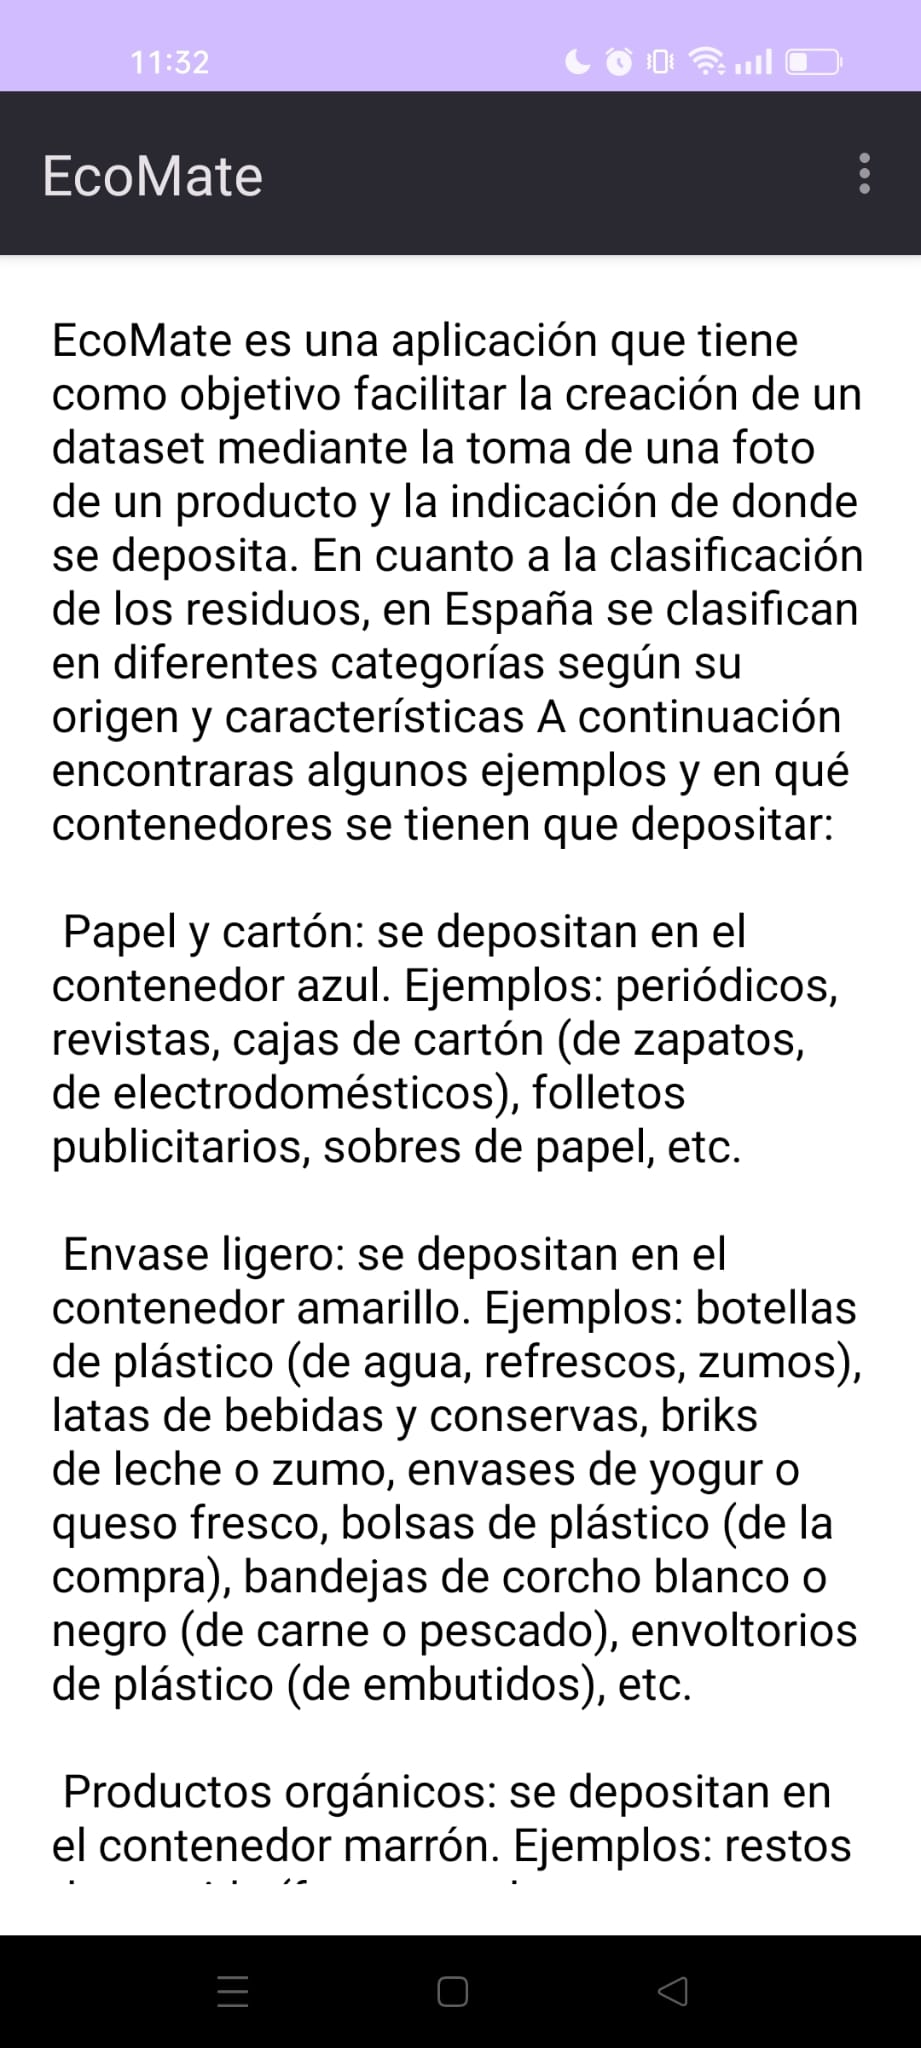
\includegraphics[width=\textwidth]{img/app_manual.jpeg}
    \caption{Manual de uso}
    \label{fig:imagen4}
  \end{subfigure}
  \begin{subfigure}[b]{0.16\textwidth}
    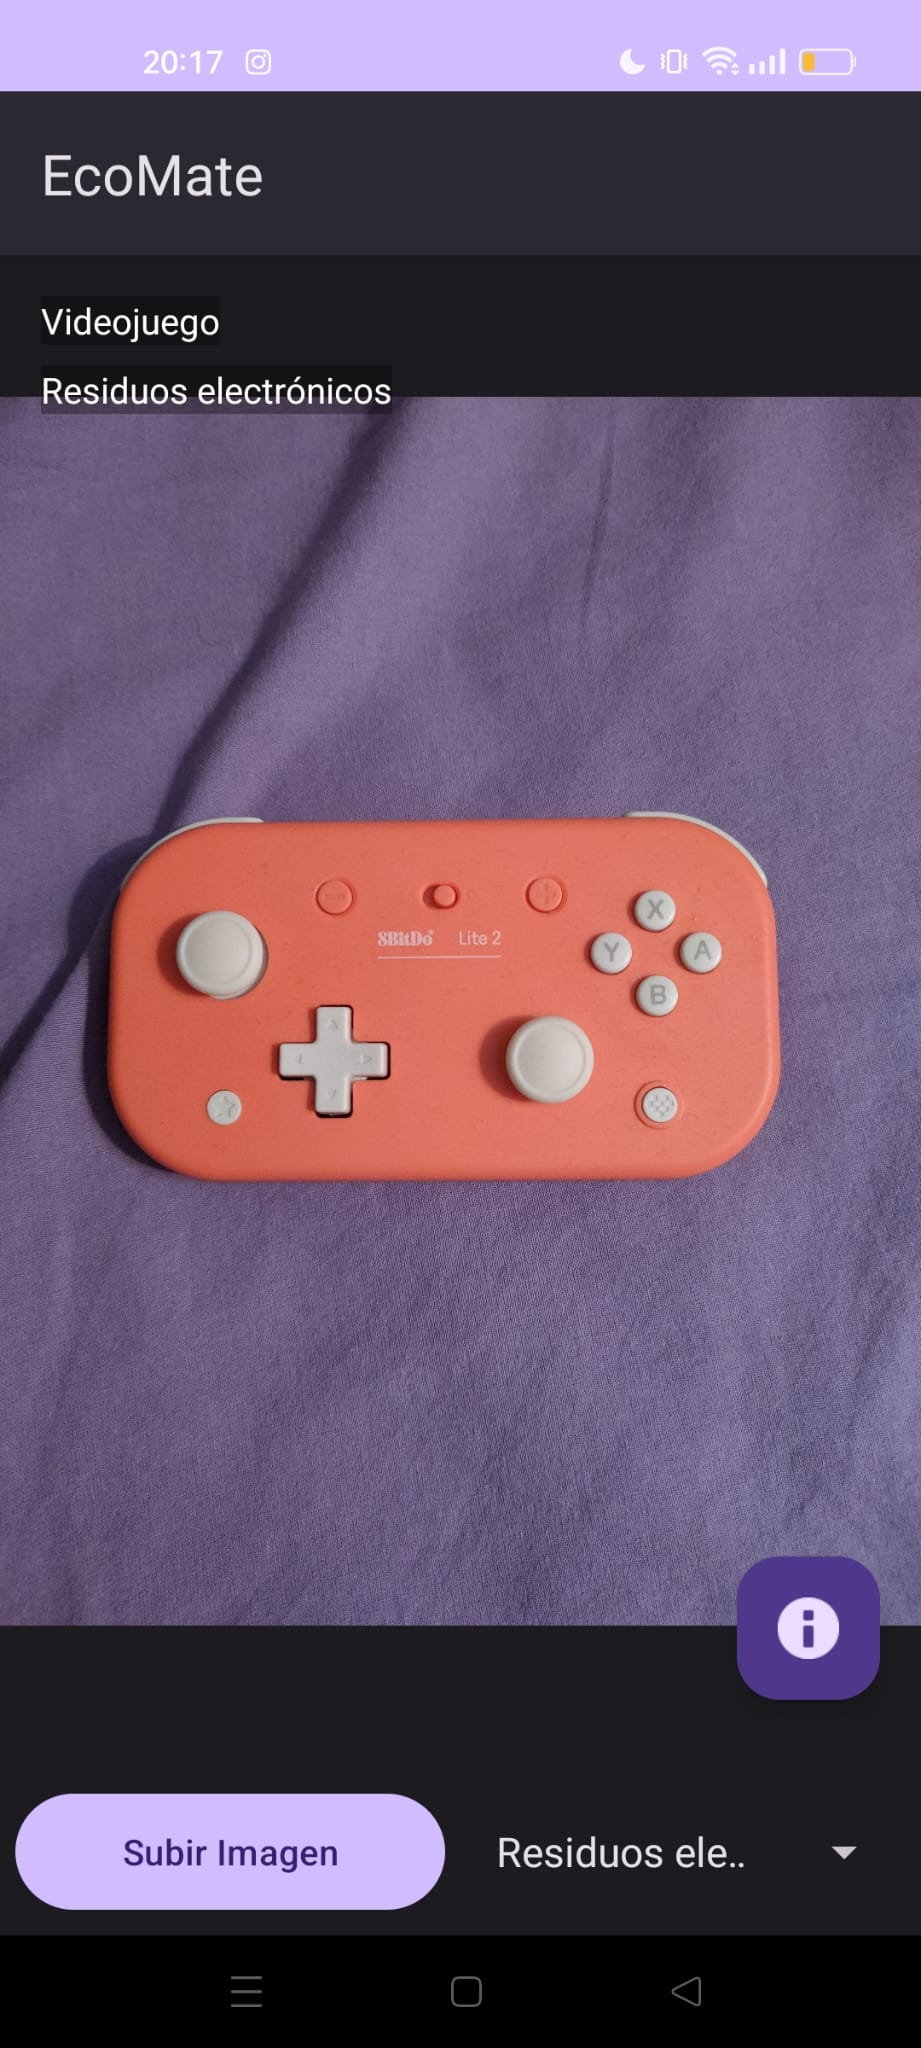
\includegraphics[width=\textwidth]{img/new_app1.jpeg}
    \caption{Clasificación}
    \label{fig:imagen5}
  \end{subfigure}
  \begin{subfigure}[b]{0.16\textwidth}
    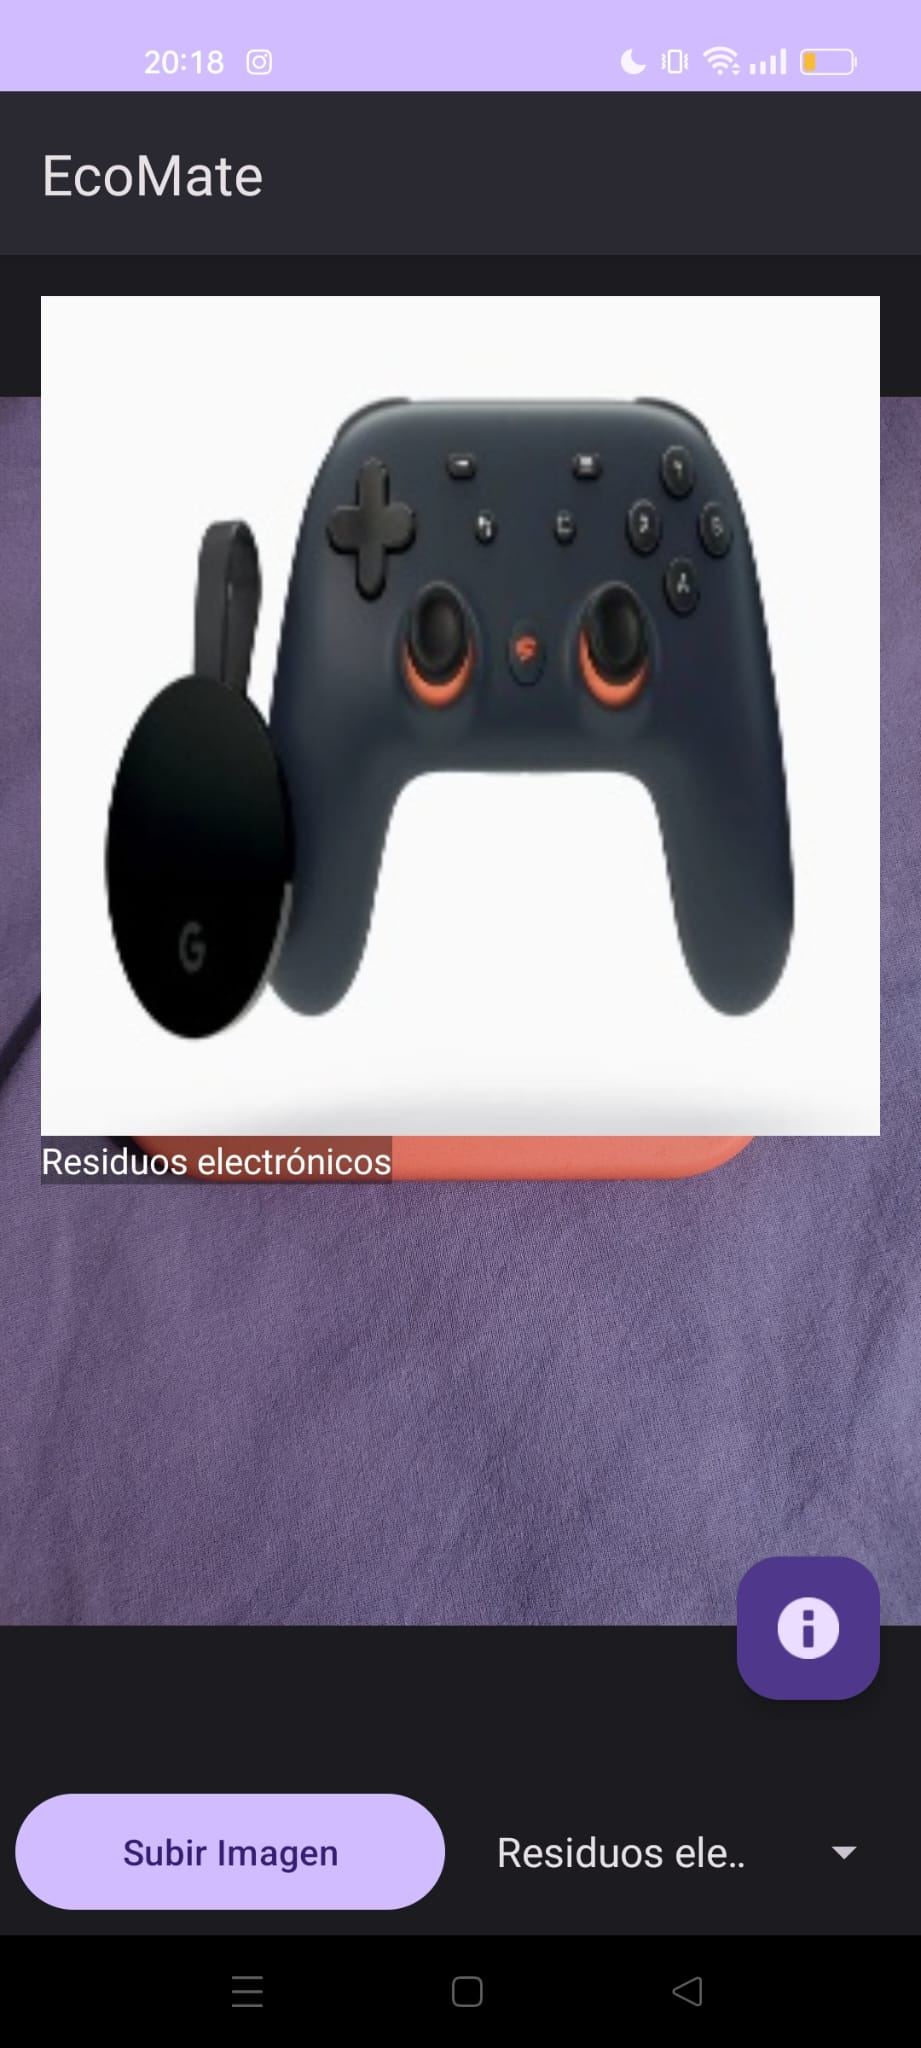
\includegraphics[width=\textwidth]{img/new_app2.jpeg}
    \caption{Imagen similar}
    \label{fig:imagen6}
  \end{subfigure}
  \caption{Interfaz de la aplicación Android.}
  \label{fig:seis_imagenes}
\end{figure}

\subsection{Modelos de clasificación}

\begin{table}[h]
  \centering
  \begin{tabular}{@{}lllllllll@{}}
  \toprule
  \textbf{Model}                      & \textbf{Train acc} & \textbf{Train loss} & \textbf{Val acc} & \textbf{Val loss} & \textbf{Params} & \textbf{Epochs} & \textbf{Time (s)/Epoch} & \textbf{Time (s)} \\
  \midrule
  convnexttiny\_no\_freeze            & 0.57                    & 1.17                & 0.91                  & 0.36              & 66.37M          & 12              & 1799.02                 & 21588.27          \\
  xception\_fine\_no\_freeze          & 0.62                    & 1.07                & 0.90                  & 0.36              & 123.63M         & 10              & 670.20                  & 6702.02           \\
  xception\_fine\_no\_freeze\_no\_aug & 0.99                    & 0.02                & 0.90                  & 0.53              & 123.63M         & 6               & 808.19                  & 4849.13           \\
  inceptionresnetv2\_no\_freeze       & 0.65                    & 0.98                & 0.90                  & 0.39              & 93.67M          & 12              & 1306.87                 & 15682.44          \\
  inceptionv3\_no\_freeze             & 0.56                    & 1.20                & 0.89                  & 0.42              & 74.24M          & 19              & 684.87                  & 13012.54          \\
  densenet121\_no\_freeze             & 0.55                    & 1.22                & 0.89                  & 0.42              & 58.43M          & 13              & 1050.03                 & 13650.33          \\
  mobilenetv2\_no\_freeze\_no\_aug    & 1.00                    & 0.02                & 0.88                  & 0.70              & 66.49M          & 10              & 335.72                  & 3357.20           \\
  mobilenetv2\_no\_freeze             & 0.58                    & 1.15                & 0.88                  & 0.44              & 66.49M          & 15              & 358.09                  & 5371.32           \\
  nasnetmobile\_no\_freeze            & 0.60                    & 1.10                & 0.87                  & 0.54              & 57.27M          & 13              & 789.63                  & 10265.25          \\
  resnet50v2\_f\_no\_freeze           & 0.55                    & 1.22                & 0.86                  & 0.54              & 126.34M         & 17              & 649.03                  & 11033.57          \\
  mobilenetv3large\_no\_freeze        & 0.56                    & 1.20                & 0.86                  & 0.52              & 51.18M          & 18              & 352.28                  & 6341.13           \\
  vgg16\_no\_freeze                   & 0.54                    & 1.25                & 0.84                  & 0.56              & 40.42M          & 22              & 689.81                  & 15175.75          \\
  resnet50\_no\_freeze                & 0.55                    & 1.22                & 0.84                  & 0.57              & 126.36M         & 14              & 698.19                  & 9774.64           \\
  xception                            & 0.93                    & 0.22                & 0.83                  & 0.69              & 123.63M         & 5               & 280.99                  & 1404.95           \\
  inceptionresnetv2                   & 0.92                    & 0.23                & 0.83                  & 0.78              & 93.67M          & 6               & 510.01                  & 3060.03           \\
  nasnetmobile                        & 0.92                    & 0.26                & 0.81                  & 0.73              & 57.27M          & 4               & 263.30                  & 1053.21           \\
  densenet121                         & 0.91                    & 0.28                & 0.81                  & 0.76              & 58.43M          & 4               & 296.39                  & 1185.57           \\
  resnet50v2                          & 0.93                    & 0.24                & 0.81                  & 1.10              & 126.34M         & 4               & 291.10                  & 1164.40           \\
  mobilenetv2                         & 0.95                    & 0.18                & 0.80                  & 1.06              & 66.49M          & 4               & 114.87                  & 459.49            \\
  mobilenetv3small\_no\_freeze        & 0.54                    & 1.25                & 0.80                  & 0.74              & 29.85M          & 24              & 201.78                  & 4842.67           \\
  inceptionv3                         & 0.93                    & 0.21                & 0.80                  & 0.92              & 74.24M          & 6               & 276.80                  & 1660.82           \\
  nasnetlarge\_aug                    & 0.92                    & 0.24                & 0.79                  & 1.02              & 287.24M         & 5               & 1025.08                 & 5125.40           \\
  xception\_aug                       & 0.65                    & 1.02                & 0.75                  & 0.84              & 123.63M         & 14              & 280.99                  & 3933.85           \\
  vgg16\_pre                          & 0.96                    & 0.12                & 0.74                  & 1.36              & 40.42M          & 8               & 221.76                  & 1774.11           \\
  vgg19                               & 0.91                    & 0.27                & 0.71                  & 1.34              & 45.73M          & 6               & 228.42                  & 1370.51           \\
  vgg16\_pre\_no\_freeze              & 0.65                    & 0.96                & 0.59                  & 1.48              & 40.42M          & 9               & 727.05                  & 6543.48           \\
  simple\_cnn                         & 0.97                    & 0.11                & 0.54                  & 3.78              & 44.4M           & 7               & 184.61                  & 1292.26           \\
  convnexttiny                        & 0.73                    & 0.77                & 0.53                  & 1.67              & 66.37M          & 6               & 727.44                  & 4364.65           \\
  convnextsmall                       & 0.66                    & 1.01                & 0.52                  & 1.61              & 88.0M           & 10              & 1164.44                 & 11644.40          \\
  mobilenetv3large                    & 0.51                    & 1.43                & 0.42                  & 1.76              & 51.18M          & 13              & 126.94                  & 1650.24           \\
  resnet50                            & 0.51                    & 1.44                & 0.35                  & 1.93              & 126.36M         & 15              & 309.29                  & 4639.32           \\
  mobilenetv3small                    & 0.37                    & 1.80                & 0.34                  & 1.89              & 29.85M          & 14              & 84.99                   & 1189.87           \\
  simple\_mlp                         & 0.38                    & 1.76                & 0.33                  & 1.95              & 77.24M          & 22              & 71.35                   & 1569.77           \\
  efficientnetv2b0                    & 0.15                    & 2.27                & 0.11                  & 2.31              & 70.16M          & 4               & 194.60                  & 778.41            \\
  vgg19\_no\_freeze                   & 0.15                    & 2.27                & 0.11                  & 2.31              & 45.73M          & 8               & 774.15                  & 6193.17           \\
  \bottomrule
  \end{tabular}
  \caption{Resultados de la evaluación de los modelos de redes neuronales.}
  \label{tab:models_full}
\end{table}

Para la red neuronal simple\_mlp se utilizó la arquitectura mostrada en la Tabla \ref{tab:arqsimplemlp}.

\begin{table}[h]
  \centering
  \begin{tabular}{>{\centering\arraybackslash}m{3cm} >{\centering\arraybackslash}m{3cm} >{\centering\arraybackslash}m{3cm}}
  \toprule
  \textbf{Capa} & \textbf{Tipo} & \textbf{Parámetros} \\
  \midrule
  Entrada & Aplanar (Flatten) & (224, 224, 3) \\
  \midrule
  Capa Densa 1 & Densa (Dense) & 512, activación='relu' \\
  \midrule
  Capa Densa 2 & Densa (Dense) & 256, activación='relu' \\
  \midrule
  Capa Densa 3 & Densa (Dense) & 128, activación='relu' \\
  \midrule
  Capa de Salida & Densa (Dense) & 10, activación='softmax' \\
  \bottomrule
  \end{tabular}
  \caption{Arquitectura de la red neuronal simple\_mlp}
  \label{tab:arqsimplemlp}
\end{table}

Para la red neuronal simple\_cnn se utilizó la arquitectura mostrada en la Tabla \ref{tab:simplecnn}.

\begin{table}[h]
  \centering
  \begin{tabular}{>{\centering\arraybackslash}m{3cm} >{\centering\arraybackslash}m{3cm} >{\centering\arraybackslash}m{4cm}}
  \toprule
  \textbf{Capa} & \textbf{Tipo} & \textbf{Parámetros} \\
  \midrule
  Entrada & Convolución 2D & 32, (3, 3), activación='relu', input\_shape=(224, 224, 3) \\
  \midrule
  Capa Max-Pooling 1 & MaxPooling2D & 2, 2 \\
  \midrule
  Capa Convolución 2 & Convolución 2D & 64, (3, 3), activación='relu' \\
  \midrule
  Capa Max-Pooling 2 & MaxPooling2D & 2, 2 \\
  \midrule
  Capa Convolución 3 & Convolución 2D & 128, (3, 3), activación='relu' \\
  \midrule
  Capa Max-Pooling 3 & MaxPooling2D & 2, 2 \\
  \midrule
  Capa Aplanar & Aplanar (Flatten) & - \\
  \midrule
  Capa Densa 1 & Densa (Dense) & 512, activación='relu' \\
  \midrule
  Capa de Salida & Densa (Dense) & 10, activación='softmax' \\
  \bottomrule
  \end{tabular}
  \caption{Arquitectura de la red neuronal simple\_cnn}
  \label{tab:simplecnn}
  \end{table}

Para las redes convolucionales pre-entrenadas se ha usado la misma arquitectura, solo ha cambiado
el modelo convolucional base. La arquitectura de las redes convolucionales se encuentra en la Tabla \ref{tab:arqconv}.

\begin{table}[h]
  \centering
  \begin{tabular}{>{\centering\arraybackslash}m{3cm} >{\centering\arraybackslash}m{3cm} >{\centering\arraybackslash}m{4cm}}
  \toprule
  \textbf{Capa} & \textbf{Tipo} & \textbf{Parámetros} \\
  \midrule
  Base ConvNetwork & ConvNetwork & ConvNetwork \\
  \midrule
  Capa Aplanar & Aplanar (Flatten) & - \\
  \midrule
  Capa Densa 1 & Densa (Dense) & 1024, activación='relu' \\
  \midrule
  Capa de Salida & Densa (Dense) & 10, activación='softmax' \\
  \bottomrule
  \end{tabular}
  \caption{Arquitectura usada para las distintas redes convolucionales.}
  \label{tab:arqconv}
\end{table}

\subsection{Prompts para OpenCLIP}

Los prompts usados para OpenCLIP se encuentran en la Tabla \ref{tab:promps_a}.

\begin{table}[h]
  \begin{tabular}{lcccccccccc}
  \hline
  Prompt                                          & Amarillo      & Azul          & Marrón        & Medica        & Pilas         & Punto         & RAEE          & Resta         & Ropa          & Verde         \\ \hline
  \{\}                                            & 0.78          & 0.63          & 0.53          & 0.44          & \textbf{0.98} & 0.76          & 0.93          & 0.70          & 0.61          & 0.70          \\
  a   photo of \{\}                               & 0.80          & 0.64          & 0.62          & 0.48          & \textbf{0.98} & 0.79          & 0.94          & 0.75          & 0.80          & 0.73          \\
  a   picture of \{\}                             & 0.77          & 0.60          & 0.42          & 0.49          & \textbf{0.98} & 0.80          & 0.95          & 0.70          & 0.79          & 0.79          \\
  a   photo of a \{\}                             & 0.83          & 0.62          & 0.70          & 0.50          & 0.97          & 0.81          & 0.95          & 0.65          & \textbf{0.81} & 0.77          \\
  a   picture of a \{\}                           & 0.83          & 0.60          & 0.59          & 0.48          & \textbf{0.98} & 0.81          & 0.95          & 0.67          & 0.76          & \textbf{0.80} \\
  an   image of \{\}                              & 0.81          & 0.56          & 0.79          & 0.44          & \textbf{0.98} & 0.79          & 0.93          & \textbf{0.79} & 0.80          & 0.71          \\
  an   image of a \{\}                            & \textbf{0.86} & 0.58          & 0.76          & 0.46          & 0.97          & 0.82          & 0.96          & 0.64          & 0.78          & \textbf{0.80} \\
  a bright photo of a \{\}                        & 0.84          & 0.66          & 0.70          & 0.47          & 0.96          & 0.80          & 0.95          & 0.59          & 0.73          & 0.75          \\
  a photo of \{\}, a type of waste                & 0.77          & 0.67          & 0.63          & 0.66          & 0.94          & 0.78          & 0.96          & 0.63          & 0.80          & 0.77          \\
  a   picture of \{\}, a type of waste            & 0.77          & 0.67          & 0.60          & 0.69          & 0.94          & 0.80          & 0.95          & 0.62          & 0.79          & 0.77          \\
  a   photo of a \{\}, a type of waste            & 0.80          & 0.67          & 0.74          & 0.65          & 0.95          & 0.81          & 0.95          & 0.64          & 0.80          & 0.77          \\
  a   picture of a \{\}, a type of waste          & 0.81          & 0.68          & 0.72          & 0.67          & 0.95          & 0.82          & 0.95          & 0.63          & 0.80          & \textbf{0.80} \\
  an   image of \{\}, a type of waste             & 0.77          & 0.64          & 0.74          & 0.58          & 0.90          & 0.80          & 0.96          & 0.63          & 0.80          & 0.77          \\
  an   image of a \{\}, a type of waste           & 0.81          & 0.67          & 0.78          & 0.63          & 0.93          & 0.81          & 0.96          & 0.62          & \textbf{0.81} & 0.78          \\
  a bright photo of a \{\}, a type of waste       & 0.83          & \textbf{0.69} & \textbf{0.82} & 0.66          & 0.93          & \textbf{0.84} & \textbf{0.97} & 0.58          & 0.80          & 0.73          \\
  a photo of \{\}, a type of domestic waste       & 0.77          & 0.67          & 0.66          & 0.67          & 0.91          & 0.79          & \textbf{0.97} & 0.69          & \textbf{0.81} & 0.74          \\
  a   picture of \{\}, a type of domestic waste   & 0.77          & 0.67          & 0.66          & \textbf{0.71} & 0.94          & 0.80          & 0.96          & 0.65          & 0.80          & 0.76          \\
  a   photo of a \{\}, a type of domestic waste   & 0.80          & 0.67          & 0.73          & 0.68          & 0.92          & 0.81          & 0.96          & 0.67          & \textbf{0.81} & 0.76          \\
  a   picture of a \{\}, a type of domestic waste & 0.79          & 0.67          & 0.76          & 0.67          & 0.94          & 0.82          & 0.95          & 0.64          & 0.80          & 0.78          \\
  an   image of \{\}, a type of domestic waste    & 0.78          & 0.64          & 0.73          & 0.60          & 0.89          & 0.80          & \textbf{0.97} & 0.67          & \textbf{0.81} & 0.77          \\
  an   Image of a \{\}, a type of domestic waste  & 0.81          & 0.65          & 0.76          & 0.65          & 0.91          & 0.80          & 0.95          & 0.65          & \textbf{0.81} & 0.75          \\
  a bright photo of a \{\}, a type of domestic..  & 0.81          & \textbf{0.69} & 0.73          & 0.67          & 0.89          & 0.82          & \textbf{0.97} & 0.60          & \textbf{0.81} & 0.71          \\ \hline
  \end{tabular}
  \caption{Resultados de los distintos promps para el modelo OpenCLIP, con los datos de validación.}
  \label{tab:promps_a}
  \end{table}


\end{document}

